\documentclass[size=a4, parskip=half, titlepage=false, toc=flat, toc=bib, 12pt, twoside]{scrartcl}

% ---------------------------------------------------------------------------
%  PAQUETES
% ---------------------------------------------------------------------------

% IDIOMA
\usepackage[utf8]{inputenc}

% MATEMÁTICAS
\usepackage{amsmath}    % Paquete básico de matemáticas
\usepackage{amssymb}	% Fuentes matemáticas
\usepackage{mathtools}
%\usepackage{upgreek}
\usepackage{amsthm}     % Teoremas
\usepackage{mathrsfs}   % Fuente para ciertas letras utilizadas en matemáticas
\usepackage{bm}

\usepackage{tgpagella}  % text only
\usepackage{mathpazo}   % math & text


% LISTAS
\usepackage{enumitem}       % Mejores listas
\setlist{leftmargin=.5in}   % Especifica la indentación para las listas.

% Dibujos Tikz
\usepackage{pgf,tikz}
\usepackage{tkz-euclide}
%\usetkzobj{all}
\usepackage{mathrsfs}
\usetikzlibrary{arrows, calc,intersections,through,backgrounds}

% Títulos de figuras
\usepackage{capt-of}

% Posición de figuras
\usepackage{float}

% ---------------------------------------------------------------------------
%  RECURSOS
% ---------------------------------------------------------------------------

% Ruta donde buscar gráficos
\graphicspath{{../_assets/}, {_assets/}, {./img/}, {ALGI/img/}, {ALGI/}}

% ---------------------------------------------------------------------------
% ENTORNOS PERSONALIZADOS
% ---------------------------------------------------------------------------

%% DEFINICIONES DE LOS ESTILOS

% Nuevo estilo para definiciones
\newtheoremstyle{definition-style}  % Nombre del estilo
{}                                  % Espacio por encima
{}                                  % Espacio por debajo
{}                                  % Fuente del cuerpo
{}                                  % Identación
{\bfseries\tgpaella}                      % Fuente para la cabecera
{.}                                 % Puntuación tras la cabecera
{.5em}                              % Espacio tras la cabecera
{\thmname{#1}\thmnumber{ #2}\thmnote{ (#3)}}  % Especificación de la cabecera

% Nuevo estilo para notas
\newtheoremstyle{remark-style}
{10pt}
{10pt}
{}
{}
{\itshape \tgpaella}
{.}
{.5em}
{}

% Nuevo estilo para teoremas y proposiciones
\newtheoremstyle{theorem-style}
{}
{}
{}
{}
{\bfseries \tgpaella}
{.}
{.5em}
{\thmname{#1}\thmnumber{ #2}\thmnote{ (#3)}}

% Nuevo estilo para ejemplos
\newtheoremstyle{example-style}
{10pt}
{10pt}
{}
{}
{\bfseries \tgpaella}
{}
{.5em}
{\thmname{#1}\thmnumber{ #2.}\thmnote{ #3.}}

% Nuevo estilo para la demostración

\makeatletter
\renewenvironment{proof}[1][\proofname] {\par\pushQED{\qed}\normalfont\topsep6\p@\@plus6\p@\relax\trivlist\item[\hskip\labelsep\itshape\tgpaella#1\@addpunct{.}]\ignorespaces}{\popQED\endtrivlist\@endpefalse}
\makeatother

%% ASIGNACIÓN DE LOS ESTILOS

% Teoremas, proposiciones y corolarios
\theoremstyle{theorem-style}
\newtheorem{nth}{Teorema}[section]
\newtheorem{nprop}{Proposición}[section]
\newtheorem{ncor}{Corolario}[section]
\newtheorem{nlema}{Lema}[section]

% Definiciones
\theoremstyle{definition-style}
\newtheorem{ndef}{Definición}[section]

% Notas
\theoremstyle{remark-style}
\newtheorem*{nota}{Nota}

% Ejemplos
\theoremstyle{example-style}
\newtheorem{ejemplo}{Ejemplo}[section]

% Ejercicios y solución
\theoremstyle{definition-style}
\newtheorem{ejer}{Ejercicio}[section]

\theoremstyle{remark-style}
\newtheorem*{sol}{Solución}

% ---------------------------------------------------------------------------
% COMANDOS PERSONALIZADOS
% ---------------------------------------------------------------------------

% Números enteros: \ent
\providecommand{\ent}{\mathbb{Z}}

% Números racionales: \rac
\providecommand{\rac}{\mathbb{Q}}

% Números naturales: \nat
\providecommand{\nat}{\mathbb{N}}


% Valor absoluto: \abs{}
\providecommand{\abs}[1]{\lvert#1\rvert}

% Fracción grande: \ddfrac{}{}
\newcommand\ddfrac[2]{\frac{\displaystyle #1}{\displaystyle #2}}

% Texto en negrita en modo matemática: \bm{}
\newcommand{\bm}[1]{\boldsymbol{#1}}

% Línea horizontal.
\newcommand{\horrule}[1]{\rule{\linewidth}{#1}}

% Restricción de una aplicación.
\newcommand\restr[2]{{% we make the whole thing an ordinary symbol
  \left.\kern-\nulldelimiterspace % automatically resize the bar with \right
  #1 % the function
  \vphantom{\big|} % pretend it's a little taller at normal size
  \right|_{#2} % this is the delimiter
  }}

% Imagen de una aplicación.
\DeclareMathOperator*{\img}{img}

% Divisores de un elemento de un anillo
\DeclareMathOperator*{\rdiv}{div}

% Listas ordenadas con números romanos (i), (ii), etc.
\newenvironment{nlist}
{\begin{enumerate}
    \renewcommand\labelenumi{(\emph{\roman{enumi})}}}
  {\end{enumerate}}

% División por casos con llave a la derecha.
\newenvironment{rcases}
{\left.\begin{aligned}}
    {\end{aligned}\right\rbrace}


% ---------------------------------------------------------------------------
%  COLORES
% ---------------------------------------------------------------------------

\usepackage{xcolor}     % Permite definir y utilizar colores

\definecolor{50}{HTML}{FFEBEE}
\definecolor{300}{HTML}{E57373}
\definecolor{500}{HTML}{F44336}
\definecolor{700}{HTML}{D32F2F}
\definecolor{900}{HTML}{B71C1C}


\setuptoc{toc}{leveldown}

% Ajuste de las líneas y párrafos
\linespread{1.2}
\setlength{\parindent}{0pt}
\setlength{\parskip}{12pt}

% Español
\usepackage[spanish, es-tabla]{babel}

% Matemáticas
\usepackage{amsmath}
\usepackage{amsthm}

% Links
%\usepackage{hyperref}

% Fuentes
%\usepackage{newpxtext,newpxmath}
\usepackage[scale=.9]{FiraMono}
\usepackage{FiraSans}
\usepackage[T1]{fontenc}

\defaultfontfeatures{Ligatures=TeX,Numbers=Lining}
\usepackage[activate={true,nocompatibility},final,tracking=true,factor=1100,stretch=10,shrink=10]{microtype}
\SetTracking{encoding={*}, shape=sc}{0}

\usepackage{graphicx}
\usepackage{float}

% Mejores tablas
\usepackage{booktabs}
\usepackage{multirow}

\usepackage{adjustbox}

% COLORES

\usepackage{xcolor}

\definecolor{verde}{HTML}{007D51}
\definecolor{esmeralda}{HTML}{045D56}
\definecolor{salmon}{HTML}{FF6859}
\definecolor{amarillo}{HTML}{FFAC12}
\definecolor{morado}{HTML}{A932FF}
\definecolor{azul}{HTML}{0082FB}
\definecolor{error}{HTML}{b00020}

% ENTORNOS
\usepackage[skins, listings, theorems]{tcolorbox}

\newtcolorbox{recuerda}{
  enhanced,
%  sharp corners,
  frame hidden,
  colback=black!10,
	lefttitle=0pt,
  coltitle=black,
  fonttitle=\bfseries\tgpaella\scshape,
  titlerule=0.8mm,
  titlerule style=black,
  title=\raisebox{-0.6ex}{\small RECUERDA}
}

\newtcolorbox{nota}{
  enhanced,
%  sharp corners,
  frame hidden,
  colback=black!10,
	lefttitle=0pt,
  coltitle=black,
  fonttitle=\bfseries\tgpaella\scshape,
  titlerule=0.8mm,
  titlerule style=black,
  title=\raisebox{-0.6ex}{\small NOTA}
}

\newtcolorbox{error}{
  enhanced,
%  sharp corners,
  frame hidden,
  colback=error!10,
	lefttitle=0pt,
  coltitle=error,
  fonttitle=\bfseries\tgpaella\scshape,
  titlerule=0.8mm,
  titlerule style=error,
  title=\raisebox{-0.6ex}{\small ERROR}
}

\newtcblisting{shell}{
  enhanced,
  colback=black!10,
  colupper=black,
  frame hidden,
  opacityback=0,
  coltitle=black,
  fonttitle=\bfseries\tgpaella\scshape,
  %titlerule=0.8mm,
  %titlerule style=black,
  %title=Consola,
  listing only,
  listing options={
    style=tcblatex,
    language=sh,
    breaklines=true,
    postbreak=\mbox{\textcolor{black}{$\hookrightarrow$}\space},
    emph={jmml@UbuntuServer, jmml@CentOS},
    emphstyle={\bfseries},
  },
}

\newtcbtheorem[number within=section]{teor}{\small TEOREMA}{
  enhanced,
  sharp corners,
  frame hidden,
  colback=white,
  coltitle=black,
  fonttitle=\bfseries\tgpaella,
  %separator sign=\raisebox{-0.65ex}{\Large\MI\symbol{58828}},
  description font=\itshape
}{teor}

\newtcbtheorem[number within=section]{prop}{\small PROPOSICIÓN}{
  enhanced,
  sharp corners,
  frame hidden,
  colback=white,
  coltitle=black,
  fonttitle=\bfseries\tgpaella,
  %separator sign=\raisebox{-0.65ex}{\Large\MI\symbol{58828}},
  description font=\itshape
}{prop}

\newtcbtheorem[number within=section]{cor}{\small COROLARIO}{
  enhanced,
  sharp corners,
  frame hidden,
  colback=white,
  coltitle=black,
  fonttitle=\bfseries\tgpaella,
  %separator sign=\raisebox{-0.65ex}{\Large\MI\symbol{58828}},
  description font=\itshape
}{cor}

\newtcbtheorem[number within=section]{defi}{\small DEFINICIÓN}{
  enhanced,
  sharp corners,
  frame hidden,
  colback=white,
  coltitle=black,
  fonttitle=\bfseries\tgpaella,
  %separator sign=\raisebox{-0.65ex}{\Large\MI\symbol{58828}},
  description font=\itshape
}{defi}

\newtcbtheorem{ejer}{\small EJERCICIO}{
  enhanced,
  sharp corners,
  frame hidden,
  left=0mm,
  right=0mm,
  colback=white,
  coltitle=black,
  fonttitle=\bfseries\tgpaella,
  %separator sign=\raisebox{-0.65ex}{\Large\MI\symbol{58828}},
  description font=\itshape,
  nameref/.style={},
}{ejer}

% CÓDIGO
\usepackage{listings}

% CABECERAS
\pagestyle{headings}
\setkomafont{pageheadfoot}{\normalfont\normalcolor\tgpaella\small}
\setkomafont{pagenumber}{\normalfont\tgpaella}

% ALGORITMOS
\usepackage[vlined,linesnumbered]{algorithm2e}

% Formato de los pies de figura
\setkomafont{captionlabel}{\scshape}
\SetAlCapFnt{\normalfont\scshape}
\SetAlgorithmName{Algoritmo}{Algoritmo}{Lista de algoritmos}

% BIBLIOGRAFÍA
%\usepackage[sorting=none]{biblatex}
%\addbibresource{bibliografia.bib}

% REFERENCIAS
\usepackage[bookmarks = true, colorlinks=true, linkcolor = black, citecolor = black, menucolor = black, urlcolor = black]{hyperref}

\renewcommand{\proofname}{\normalfont\tgpaella\bfseries\small DEMOSTRACIÓN}

\title{Método de ranking en el diseño de un sistema de acceso a la información}
\subject{Trabajo de fin de grado}
\author{Johanna Capote Robayna\\
    Doble Grado en Ingeniería Informática y Matemáticas}
\date{}
\publishers{\vspace{2cm}
\includegraphics[height=2.5cm]{UGR}
\vfill
\vspace{2cm}
\Large
Facultad de Ciencias \\
E.T.S de Ingeniería Informática y de Telecomunicación\\
\vspace{2cm}
\Large

Tutoras: \\
Silvia Acid Carrillo \\
Margarita Arias López}


\begin{document}
\maketitle
\thispagestyle{empty}

\newpage
\thispagestyle{empty}
\afterpage{\null\newpage}

\newpage
\section*{Agradecimientos}
\thispagestyle{empty}

\vspace{1cm}

Quiero agradecer a la Universidad de Granada por darme la oportunidad de formarme en estos estudios y a todos y cada uno de los profesores que me han impartido clase a lo largo de estos cinco años, ya que cada uno de ellos con sus enseñanzas han contribuido en mi formación.

A mis tutoras, Margarita Arias y Silvia Acid, por su esfuerzo y dedicación, quienes con sus conocimientos y experiencias han logrado motivarme para que yo pueda llevar a cabo este trabajo.

A mis amigos y compañeros de carrera, por estar siempre ahí, alegrándose conmigo en los buenos momentos y consolándome en los malos. Por su amistad incondicional, porque gracias a ellos, estos cinco años serán un recuerdo inolvidable y formarán una parte importante de mi vida.

Y por último y no menos importante, a mi familia, sin cuyo apoyo no habría podido realizado estos estudios y quienes me han ayudado a sobrellevar estos meses de confinamiento.

\newpage
\thispagestyle{empty}
\afterpage{\null\newpage}

\newpage

\pagestyle{empty}
\tableofcontents
\clearpage
\pagestyle{headings}
\newpage

\section{Resumen}
El objetivo de este trabajo es estudiar y entender el funcionamiento del algoritmo PageRank, además se implementa un buscador, cuya base es este algoritmo, que en respuesta a una consulta consiga recuperar información útil para el usuario dentro de una colección grande de documentos en los que podría estar potencialmente interesado.

La parte matemática se centra en el teorema de Perron-Frobenius para matrices no negativas. Este resultado permite determinar cuándo una matriz no negativa admite un valor propio dominante y constituye la base del algoritmo de PageRank. Se demuestra que el radio espectral de una matriz positiva es valor propio dominante y admite un vector propio con todas las entradas positivas (teorema de Perron) y se determina bajo qué condiciones se puede extender este resultado a matrices no negativas. Se estudia el comportamiento límite de las potencias de matrices con valor propio dominante y se justifica cómo este comportamiento permite aplicar un método iterativo, el conocido método de las potencias, para aproximar numéricamente el valor propio dominante y el llamado vector de Perron, cuando se trabaja con matrices de gran dimensión

Para la parte de informática se ha implementado un buscador en lenguaje python, que consigue ordenar los archivos del conjunto de datos siguiendo el algoritmo PageRank. Adicionalmente se ha implementado una interfaz de usuario para facilitar la forma de introducir las consultas y mostrar los resultados de la búsqueda. Para poder realizar consultas en el sistema se han estudiado e implementado dos modelos diferentes, el modelo booleano y el modelo vectorial. Por último, con el objetivo de realizar consultas personalizadas se han estudiado e implementado la pseudo-realimentación de consulta, la cual extiende la consulta dependiendo de los documentos que le hayan resultado relevantes al usuario que realiza la consulta.

\textbf{\underline{Palabras clave}}: PageRank, Perron-Frobenius, método de las potencias, Recuperación de Información, buscador, modelo booleano, modelo vectorial, realimentación de consultas.

\newpage

\section{Extended Abstract}
The objective of this work is to study, understand and implement the PageRank algorithm, in addition the implementation of a search engine for a specific dataset, which by means of queries manages to retrieve useful information for th user. The main problem we will deal with is how to obtain an algorithm to order a certain group of web pages with cross references among them. This order must ensure that the most relevant pages for the user appear in the first few positions of the ranking.

\underline{Maths}

For the mathematical part, a study of the model used in said algorithm has been carried out, adapting it to a problem of eigenvalues and eigenvectors. To do this, first of all, a graph has been built where the links between the web pages have been represented. Next, the importance of a web page has been defined as the sum of the importances of the pages that it cites. When constructing the adjacency matrix we realize that the problem of granting certain relevance or importance to a web page coincides with the problem of calculating a certain eigenvector of that matrix.

Once the problem has been identified in the mathematical field, we study what properties the matrices must fulfill to guarantee the existence of a solution. For this we begin with the study of matrices, where we define the key term in this work: the dominant eigenvalue of a matrix. This eigenvalue complies with being positive, greater in modulus than the rest of eigenvalues ​​and verify that its algebraic multiplicity is equal to one. The study of this dominant eigenvalue becomes interesting since the eigenvector associated with it is the solution to our problem. The study continues with positive matrices, where several propositions that we can summarize in Perron's Theorem are demonstrated, which assures us that for every positive matrix its spectral radius is the dominant eigenvalue and defines the Perron vector as the only one associated with the dominant eigenvalue with norm equal to one. This theorem would solve our problem, if our matrix were positive, since the solution to our problem would be the Perron vector. However, our matrix can have null inputs, so we continue to study non-negative matrices. Several properties that these matrices fulfill are studied and the Perron-Frobenius Theorem is proved, which ensures that every non-negative and irreducible (a property that is adequately defined) matrix always has an eigenvalue that is greater or equal in modulus than all other eigenvalues ​​and that it has a positive eigenvector associated with this eigenvalue. This vector is the solution to our initial problem. Finally, we study the method of powers, a key algorithm to approximate the solution vector of our problem, since a considerably large amount of data is used and the calculation of exact solution can be computationally expensive and many times imposible.

\underline{Computer Engineering}

For the computing part, a practical study of the algorithm has been carried out, adapting the theoretical model, obtaining a matrix with no null elements in its inputs. This model is implemented in the Python programming language and a study is carried out on a PMSC-UGR dataset. This dataset consists of 26759991 articles based on scientific articles from MEDLINE / PubMed. We extract 3,000 files from this data set, summing up to some 26,000 different words between the title, abstract and keywords. The reason for this selection is the limitation of resources, because in the attempt to implement the algorithm with all the articles the resulting matrix reached a very large dimension, preventing the computer used from operating with it.

Two models of Information Retrieval are implemented to be able to make queries about the data set. We seek through a query to show relevant information for the user. For this, two models are implemented: the Boolean model and the vectoria model.

The Boolean model is based on Boolean logic, this model only takes into account the presence of any of the query words in the document, it does not take into account the frequency or importance of the word. Documents or files are considered as sets of words. The logical operators (AND, OR and NOT) are used to structure the queries, and subsequently more complex queries can be obtained. The results of the query will be ordered according to the PageRank weights. The advantage of this model is its simplicity of implementation, as well as having great flexibility when making different queries thanks to the use of logical operators. On the other hand, only the presence of the query term is taken into account in each of the documents. This may be a mistake since there are terms that are more important than others and whose appearance in the document should increase its relevance. In addition, the frequency of each term in the documents is not taken into account, it is not the same that the word appears only once more than one appears. These drawbacks are solved in the following model.

In the vector model, a vector is built for each document and query where the terms of each one are reflected. That is, a vector space of size the number of terms in the document collection is created. To evaluate the importance of each term in the documents, a weight matrix is constructed, these weights take into account the frequency and specificity of the term in the document. Once the weights of all the terms and the query have been calculated, the similarity between the query vector and the document vectors is calculated. This similarity is calculated using the cosine distance. After these operations, a relevance vector is obtained where the similarity of each document to the query is reflected. These similarities are multiplied by the PageRank vector to obtain the new order.

Finally, a pseudo-feedback of queries is implemented, which seeks to expand the initial query entered by the user using documents that are interesting to them. From the terms of these documents, using the Rocchio formula, a new expanded query is achieved. After calculating the new query, the similarity between it and the documents is calculated again, obtaining a vector that is subsequently multiplied by the PageRank vector. The study considers that the users are the authors themselves and that the relevant documents are the written documents. One of the biggest advantages of this technique is that it is an automatic process, it does not require user intervention. However, the effectiveness of the technique depends on the goodness of the first result, if the query returns a result where the documents are relevant, the extension of the query will recover the most relevant documents, but if, on the contrary, the first recovery is not good, terms related to it will appear in the expanded query, making it less relevant to the user.

To better display the search engine results and improve communication between the user and the system, a graphical interface is developed, where the user can comfortably enter the query and view the results. You can also select the model to use and, in the case of a personalized query, choose which user is the one that performs it.

\underline{Conclusion}

In conclusion, the PageRank algorithm gets quite good results in ordering the files by relevance. In addition, the implemented models achieve good results, managing to personalize the searches.

It would be interesting, as future projects, to create user profiles with different interests in order to better personalize the search, showing in the first results the most interesting files for the user depending on their profile.

\textbf{\underline{Palabras clave}}: PageRank, Perron-Frobenius, mthod of powers, Data recovery, search engine, boolean model, vectorial model, query feedback.

\newpage

\section{Introducción}
\subsection{Contextualización}
Fue en la década de los 80 cuando Internet empezaba a darse a conocer con unas primeras páginas web \footnote{En el contexto de R.I. se suelen denominar documentos.} de estilo muy básico y sencillo que tardaban mucho en cargarse. Con el transcurso del tiempo la Red fue creciendo a pasos agigantados almacenando un gran volumen de información lo que provocó  un sinfín de procesos y cambios en las formas de gestionarla, y es en ese contexto donde surgen los buscadores para dar respuesta a la necesidad de clasificar y gestionar gran cantidad de información lo más rápido posible.

Un buscador o motor de búsqueda es un sistema de recuperación de información, donde el usuario introduce un conjunto de términos \footnote{En el contexto de R.I. se suele denominar consulta (\textit{query}).} o palabras clave y el buscador le devuelve una lista de resultados \footnote{En el contexto de R.I. los resultados son los documentos o páginas relevantes de la consulta.} ordenados bajo una serie de criterios. WebCrawler, Lycos, AltaVista o Yahoo entre otros, son los primeros buscadores de la Historia que funcionaban de una forma muy similar, rastreaban la Red y clasificaban las páginas en función de las veces que contenían las palabras clave introducidas. Eran los más utilizados en esa época hasta que en 1998 son desbancados por Google, el mayor motor de búsqueda de todos los tiempos,  que consigue imponerse al resto de buscadores gracias a un nuevo algoritmo de búsqueda (PageRank), capaz de ordenar una gran cantidad de información en poco tiempo.

PageRank es un algoritmo basado en el Álgebra lineal, Teoría de Grafos y Probabilidad, fue diseñado por Sergey Brin y Lawrence Page, el primero graduado en Matemáticas y el segundo en Informática y ambos estudiantes de doctorado de Informática de la Universidad de Standford. La pregunta que buscaban resolver era clara ``?`en qué orden mostrar los resultados de la búsqueda?''. En 1997 cuando Brin y Page empezaron a trabajar en el diseño del algoritmo se plantearon como objetivo principal que en el gran número de los casos, al menos una de las primeras páginas que se muestran como resultado contenga información útil para el usuario. Hay que tener en cuenta que en esta época Internet no era tan grande como ahora, habían censadas en torno a 100 millones de páginas web y los buscadores más famosos de la época eran capaces de atender 20 millones de consultas al día, mientras que hoy en día Google es capaz de atender a 200 millones de consultas diarias. Pasaremos a explicar cómo el algoritmo de PageRank es capaz de ordenar estas millones de páginas web en tan poco tiempo.

\subsection{Introducción al modelo}
Lo primero que hace Google, incluso antes de que el usuario realice la búsqueda es organizar el contenido de Internet ayudándose de un índice. Este índice se va actualizando y va añadiendo páginas nuevas y modificando la información de las páginas ya existentes en un proceso llamado ``rastreo'', en el cual adquiere información de esas páginas incluyendo los enlaces hacia otra páginas. El índice se ordena con el algoritmo de \textbf{PageRank}, se explicará a continuación, que ordena la lista asignando un PageRank más alto a las páginas que calificará de ``más interesantes'' y un PageRank bajo a las páginas ``menos interesantes''.

En un buscador cuando el usuario introduce su búsqueda esta pasa por varias fases \footnote{Información extraida de \url{https://www.google.com/search/howsearchworks/algorithms/}}:
\begin{itemize}
\item \textbf{Análisis de las palabras del usuario}. En esta fase se busca entender el significado de la búsqueda, para ello se analiza las palabras usadas y se interpreta lo que el usuario quiere decir con ellas. Este proceso incluye varios pasos como \textbf{interpretar los errores de ortografía} o entender el significado que el usuario le está dando a una palabra con varias acepciones ayudándose de un \textbf{sistema de sinónimos}. Otro aspecto importante de esta fase es el \textbf{algoritmo de novedades}, el cual deduce que en ciertas búsquedas debe mostrar la información más actual, como por ejemplo si el usuario busca ``horóscopo'' o ``resultados del fútbol club Granada'' se está interesando por las últimas publicaciones.
\item \textbf{Búsqueda de coincidencias}. En esta fase se busca entre las páginas del índice aquellas con información coincidente con la búsqueda. Se analiza la frecuencia con la que aparecen las palabras introducidas en las páginas web candidatas y su localización; es decir, si aparecen en el título, encabezamientos o en el cuerpo del texto. Además existen otros algoritmos que analizan si las páginas candidatas pueden resultar interesantes para el usuario, ya que si por ejemplo el usuario busca ``pájaros'' lo más probable es que no quiera encontrar una página con poca información relevante sobre el tema pero en la que se repite muchas veces la palabra ``pájaro''.
\item \textbf{Mejora del posicionamiento de las páginas útiles}. Una vez obtenidas las páginas web con información potencialmente válida se pasa a clasificar su utilidad con el objetivo de mostrar primero las páginas más útiles para el usuario. En esta fase se analizan varios factores como el número de veces que aparece el término buscado en la página, la fecha de publicación y la calidad de experiencia del usuario en la página. Además se descartan aquellos sitios web con contenido fraudulento o \textit{spam} y se potencia las páginas que en consultas similares hayan sido fiables.
\item \textbf{Devolver los mejores resultados}. En esta parte se busca la diversidad de respuestas. Antes de mostrar el resultado de la búsqueda se analiza el resultado en conjunto, se evalúa si hay muchas páginas centradas en la misma interpretación de la búsqueda o si solo existe un tema en los resultados.
\item \textbf{Análisis del contexto}. Esta fase no se realiza siempre, en ella se busca ``personalizar'' la búsqueda con datos como la ubicación o historial de búsqueda. Con ello se consigue reducir la búsqueda a su entorno, por ejemplo si el usuario es español y busca ``baloncesto'' le saldrá antes información sobre el baloncesto en España que sobre el de otros países o si el usuario busca ``conciertos cerca de mi'' aparecerán los conciertos más cercanos a su residencia. Además mediante el historial de búsqueda personal el buscador consigue mejorar la interpretación de la búsqueda, por ejemplo si el usuario ha buscado anteriormente ``Granada vs Osasuna'' y más adelante busca ``Granada'' puede considerar que el usuario se refiere al equipo de fútbol y no a la ciudad.
\end{itemize}

\newpage

\subsection{Descripción del problema}
El problema que se va a abordar en este trabajo es conseguir un método de \textit{ranking} para ordenar la información según el interés del usuario. Para ello se investigarán las ténicas utilizadas por uno de los mayores motores de búsqueda, Google, y se aplicarán sobre un conjunto de datos específico PMSC-UGR para realizar la parte experimental, que se detallará en la sección \ref{Base de datos}. Para abordar el problema nos centramos en la parte preliminar a una búsqueda. Como ya se comentó anteriormente, antes de que el usuario realice una búsqueda en Google las páginas web ya se encuentran previamente ordenadas por el algoritmo PageRank. Este algoritmo  es en el que se centrará este trabajo dividido en dos grandes partes:
\begin{itemize}
\item En la primera parte se realizará un estudio teórico del algoritmo PageRank, en el que se datallará la base matemática de manera formal. En primer lugar se ajustara nuestro problema a un problema de valores y vectores propios y a continuación se desarrollaran varios resultados matemáticos que garantizan la existencia de una solución.
\item En la segunda parte se realizará un estudio práctico del algoritmo PageRank sobre el conjunto de datos comentado, además se utilizan distintos modelos de Recuperación de Información en los cuales a partir de consultas el usuario podrá obtener documentos que le resulten relevantes o más interesantes.
\end{itemize}

\newpage

\subsection{Principales fuentes}
Las principales fuentes utilizadas son:
\begin{itemize}
\item  Carl D. Meyer.
\textit{Matrix Analysis and Applied Linear Algebra}. Siam. 2000. \cite{algebralineal}
\item Fidel Cacheda Seijo, Juan Manuel Fernández Luna y Juan Francisco Huete Guadix.
\textit{Recuperación de Información. Un enfoque práctica y multidisciplinar}. RA-MA Editorial y Publicaciones. 2011. \cite{ri}.
\end{itemize}

La mayoría de resultados de Álgebra Lineal de este trabajo han sido extraídos del primer libro, el cual desarrolla la mayoría de las propiedades, proposiciones y teoremas sobre las matrices utilizados en este trabajo. Por otro lado el segundo libro es utilizado para la parte de informática, el cual detalla los algoritmos y modelos de la Recuperación de Información, que son  estudiados e implementados en este trabajo.

\newpage

\section{Objetivos}
Como ya se comentó anteriormente el problema que se busca resolver es conseguir un método de \textit{ranking} para ordenar información según el interés del usuario. Para resolverlo se estudian e implementan algoritmos como el PageRank y varios modelos de Recuperación de Información. Por lo tanto los objetivos de este trabajo son:
\begin{itemize}
\item Demostrar la existencia de solución del problema (Teorema de Perron-Frobenius).
\item Estudiar y demostrar un método para obtener una solución aproximada (método de las potencias).
\item Implementar el algoritmo PageRank.
\item Implementar los modelos de Recuperación de Información y estudiar sus resultados.
\end{itemize}

Todos los objetivos son alcanzados.
\newpage

\section{Planificación}
En esta sección mostramos las distintas tareas desarrolladas durante el proyecto y su duración.
\begin{itemize}
\item Documentación: 2 semanas.
\item Marco teórico: 2 semanas.
\item Estudio del método de las potencias: 2 semanas.
\item Implementación del método de las potencias: 6 semanas.
\begin{itemize}
\item Implementación: 2 semanas.
\item Pruebas: 2 semanas.
\item Dudas: 2 semanas.
\end{itemize}
\item Implementación de la lectura de datos: 2 semanas.
\begin{itemize}
\item Implementación: 1 semana.
\item Pruebas y dudas: 1 semana.
\end{itemize}
\item Estudio teórico de las propiedades de las matrices positivas: 2 semanas.
\item Implementación del PageRank: 2 semanas.
\begin{itemize}
\item Implementación: 1 semana.
\item Pruebas y dudas: 1 semana.
\end{itemize}
\item Estudio teórico de las matrices no negativas: 2 semanas.
\item Implementación del modelo booleano: 4 semanas.
\begin{itemize}
\item Implementación: 2 semanas.
\item Pruebas y dudas: 2 semanas.
\end{itemize}
\item Estudio teórico del Teorema de Perron-Frobenius: 2 semanas.
\item Implementación de la interfaz gráfica: 2 semanas.
\begin{itemize}
\item Implementación: 1 semana.
\item Pruebas y dudas: 1 semana.
\end{itemize}
\item Implementación del modelo vectorial: 2 semanas.
\begin{itemize}
\item Implementación: 1 semana.
\item Pruebas y dudas: 1 semana.
\end{itemize}
\end{itemize}

La planificación temporal que se ha seguido en este trabajo es la siguiente:
\begin{center}
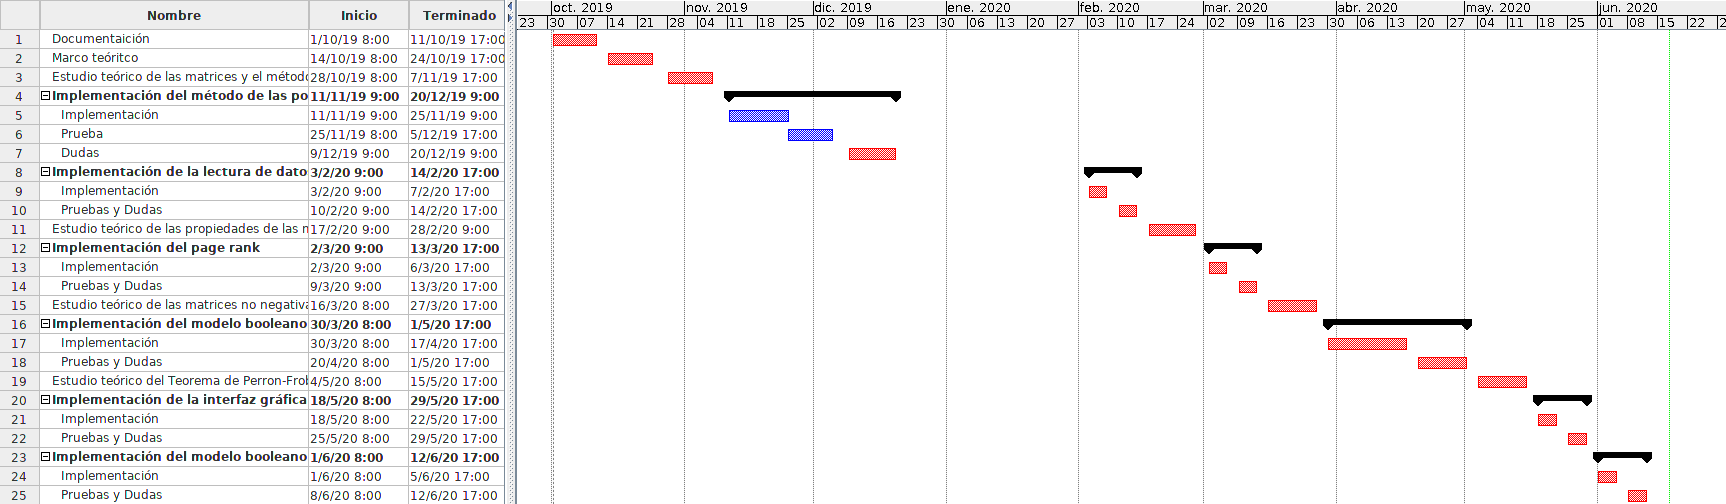
\includegraphics[width=1.1\textwidth]{grantt}
\end{center}

\newpage

\part{Matemáticas}

\section{Modelo matemático}

El algoritmo de PageRank utilizado para ordenar las páginas web tiene una base matemática de Álgebra Lineal: transformaremos el problema de ordenar las páginas web según su interés en un problema clásico de valores propios y vectores propios.

En primer lugar, vamos a definir el marco donde nos encontramos. Nuestro problema actual es establecer un criterio para ordenar las páginas de la red. Si llamamos $P_1, \dots, P_n$ a cada una de las páginas, siendo $n$ un número natural ($n \in \mathbb{N}$), definimos entonces la importancia $x_i$  de la página $P_i$ como un número real entre $0$ y $1$.

Esta importancia la utilizaremos para elegir qué páginas web son las primeras que mostramos en el buscador, ordenándolas de mayor  a menor valor de importancia.
Para calcular este número nos basamos en la información que podemos extraer de la red (sitios, contenido, enlaces de una página web a otra, etc).

En el primer modelo nos quedamos solo con los enlaces entre páginas web. Estos enlaces los podemos representar mediante un grafo dirigido (G), en el cual representamos cada $P_i$ como un nodo del grafo y por cada enlace de una página $P_i$ a $P_j$ añadimos una arista de $P_i$ a $P_j$ indicando el final con una punta de flecha, como se muestra en la imagen.

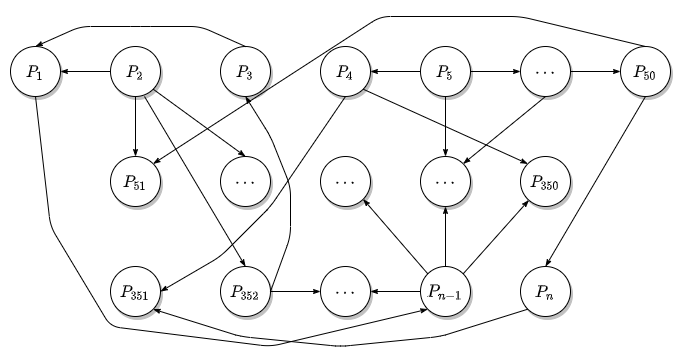
\includegraphics[width=1.0\textwidth]{./img/grafogrande}

Esta información la podemos reflejar en una matriz M de dimensión $nxn$. Tanto en las filas como en las columnas representamos las $n$ páginas y por cada enlace entre una página $j$ a otra página $i$, escribimos un $1$ en la entrada de la
matriz $m_{ij}$ y en el caso de que no haya enlace escribimos un $0$.

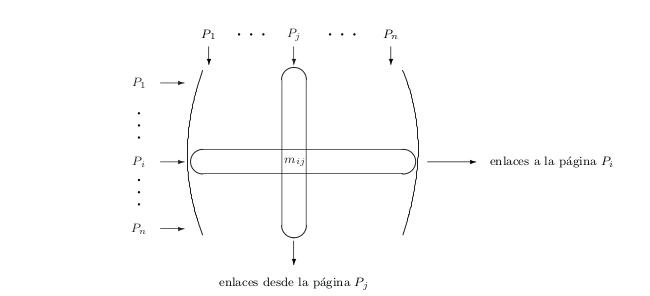
\includegraphics[width=1.0\textwidth]{./img/matriz}

Por lo tanto en la columna $j$ estarán los enlaces que salen de la página $P_j$ hacia otras páginas
mientras que en la fila $i$ estarán representados los enlaces a la página $P_i$. Esta matriz
no es simétrica ya que una página puede estar citada por otra y ella no citar a ninguna.

En una primera aproximación de querer ordenar las páginas web por ``importancia'' o ``relevancia'' podemos pensar que la página a la que le lleguen más enlaces (fila con mayor número de $1$) es la que debería mostrarse primero en el \textit{ranking}. Es decir si $x_j$ es la importancia de $P_j$, esta es proporcional al número de páginas desde las que hay enlaces a $P_j$.

Sin embargo, la realidad es que el número de enlaces a una cierta página no representa del todo su importancia, ya que no es lo mismo que esta esté citada por una página cualquiera a que esté citada desde \verb|www.facebook.com| o \verb|www.apple.com|. Estos dos últimos enlaces deberían ponderar más en importancia que otras citas de otras páginas web menos relevantes. Por lo que para asignar importancia a una página web, deberemos tener en cuenta tanto si es una \textbf{página muy citada} como si es una \textbf{página poco citada, pero de sitio ``relevantes''}.

Nos damos cuenta de que la importancia de la página citadora también es relevante, por lo que en una segunda aproximación pasamos a decidir que la importancia $x_j$ de una página $P_j$ es proporcional a la suma de las importancias de las páginas que enlazan con $P_j$. El cambio reside en que en la primera aproximación del modelo la importancia de $P_i$ era proporcional al número de páginas que enlazan con $P_i$, mientras que en esta segunda aproximación la importancia de $P_i$ es proporcional a la suma de las importancias de las páginas que enlazan con $P_i$.

Supongamos, por ejemplo, que la página $P_1$ es citada desde las páginas $P_{200}$ y $P_{n}$ ,
 que $P_2$ se cita desde $P_1$, $P_{200}$ y $P_{n-1}$ , mientas que en la última página $P_n$ hay enlaces desde $P_1$ , $P_2$ , $P_{50}$ , $P_{200}$ y $P_{n-1}$. En nuestra asignación anterior, $x_1, \dots , x_n$ deberían
 cumplir entonces que:
 $$ x_1 = K (x_{200} + x_n) $$
 $$ x_2 = K (x_1 + x_{200} + x_{n-1}) $$
 $$ \vdots $$
 $$x_n = K (x_1 + x_2 + x_{50} + x_{200} + x_{n-1}) $$

donde $K$ es una constante de proporcionalidad. Si nos fijamos, hemos construido un sistema de ecuaciones
donde las soluciones son los posibles valores de $x_1, \dots , x_n$. Este sistema de ecuaciones
lo podemos escribir en términos matriciales:

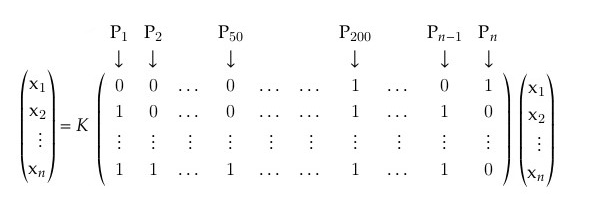
\includegraphics[width=1.0\textwidth]{./img/matrizejemplo}
Si llamamos $\vec{x}$ al vector de importacias $(x_1 \dots x_n)$, $\lambda = \frac{1}{K}$ y
$M$ a la matriz de dimensiones $n x n$ del sistema (matriz asociada al grafo). Nos encontramos
con un problema de valores propios y vectores propios:
$$M \vec{x} = \lambda \vec{x} $$

A este vector $\vec{x}$ le exigimos que sea no negativo, es decir, que todas sus componentes sean no negativas, ya que cada una de sus componentes representa la importancia de una página web y también buscamos que sea ``único'', en el sentido de que cualquier otro vector propio asociado a ese mismo valor propio sea múltiplo de este, ya que como nuestro objetivo final es establecer un \textit{ranking}, de haber dos vectores linealmente independientes tendríamos dos formas distintas de ordenar y habría que diseñar otro proceso de selección.

El estudio de la existencia de vector propio con esas propiedades para matrices con todas sus entradas no negativas es el objetivo de la Teoría de Perron-Frobenius que desarrollaremos en la siguiente sección.

\newpage

\section{Teorema de Perron-Frobenius}

Como hemos dicho anteriormente, en esta sección nos centraremos en el Teorema de Perron-Frobenius. Este resultado garantiza la existencia de un valor propio cumpliendo las propiedades que son la base del algoritmo del Pagerank.

La mayoría de los resultados aquí expuestos se pueden encontrar, por ejemplo, en \cite{algebralineal}.

En primer lugar pasamos a introducir algunas notaciones y definiciones que usaremos posteriormente.

Dadas $A = (a_{ij}),B = (b_{ij}) \in M_n(\mathbb{C})$ y $\vec{x} = (x_1, \dots, x_n)^t\in \mathbb{C}^n$:
\begin{enumerate}
\item Diremos que $A$ es no negativa si $a_{ij}\geq 0$ , $1 \leq i,j \leq n$ y lo notaremos
$A\geq 0$.
\item Diremos que $A$ es positiva si $a_{ij} > 0$ , $1 \leq i, j \leq n$ y lo notaremos $A > 0$.
\item Diremos que $B$ es mayor o igual que $A$ si $a_{ij} \leq b_{ij}$, $1 \leq i,j \leq n$ y lo notaremos $A \leq B$.
\item Diremos que el vector $\vec{x}$ es no negativo si $x_i \geq 0$ , $1 \leq i \leq n$ y lo notaremos $\vec{x} \geq 0$.
\item Análogamente diremos que el vector $\vec{x}$ es positivo si $x_i > 0$, $1 \leq i \leq n$ y lo notaremos $\vec{x} > 0$.
\end{enumerate}

Denotaremos, como es habitual:
\begin{enumerate}
\item $\sigma (A)$ al espectro de $A$, es decir $\sigma(A) = \{ \lambda \in \mathbb{C} : det(A - \lambda I)= 0\}$
\item $\rho(A)$ al radio espectral de $A$, es decir $\rho(A) = \max\{|\lambda| : \lambda \in \sigma(A) \}$.
\item $m(\lambda)$ a la multiplicidad algebraica del valor propio $\lambda$, es decir $m(\lambda)$ es la multiplicidad de $\lambda$ como raíz del polinomio característico $p(\lambda) = det(A - \lambda I)$.
\item $\nu(\lambda)$ a la multiplicidad geométrica del valor propio $\lambda$, es decir $\nu(\lambda)$ es la dimensión del subespacio propio generado por $\lambda$.
\end{enumerate}

Además llamaremos par propio a la pareja $(\lambda, \vec{x})$ donde $\lambda$ es un valor propio y $\vec{x}$ un vector propio asociado a $\lambda$.

Además de estos elementos básicos del Álgebra Lineal, también utilizaremos las formas canónicas de Jordan. La demostración de este resultado, que se estudia habitualmente en el grado, puede verse, por ejemplo en \cite{jordan}.

\begin{nth}[Forma canónica de Jordan]
Existe una matriz $P \in M_n(\mathbb{C})$, $det P \neq 0$ y $J \in M_n(\mathbb{C})$ diagonal por bloques, es decir, $J = diag(J_1, \dots, J_s)$, tales que
$$A = P J P^{-1} $$
$J$ se denomina ``forma canónica'' de $A$ y a cada unos de los bloque $J_i$, $i = 1, \dots, s$,  ``bloques elementales'' de Jordan. $J$ viene determinada por las siguientes propiedades:
\begin{enumerate}
\item Cada uno de los bloques elementales, $J_i$, está asociado a un mismo valor propio, $\lambda \in \sigma(A)$, y es de la forma:
$$J_i = \left(
      \begin{array}{{ccccc}}
        \lambda_i   &   1       &         &    & \\
              &    \lambda_i    &    1     &    & \\
              &           & \ddots  &  \ddots   & \\
              &           &         & \lambda_i & 1 \\
              &           &         &           & \lambda_i
      \end{array}
\right) = \lambda_i I_{p_i} + N_{p_i} \textrm{ siendo } N_{p_i} = \left(
      \begin{array}{{ccccc}}
            0   &   1       &         &    & \\
              &    0    &    1     &    & \\
              &           & \ddots  &  \ddots   & \\
              &           &         & 0 & 1 \\
              &           &         &           & 0
      \end{array}
\right)$$
\item Cada valor propio $\lambda$ se repite exactamente $m(\lambda)$ veces en la diagonal de $J$.
\item El número de bloques elementales correspondiente al valor propio $\lambda$ es $\nu(\lambda)$.
\item El número de bloques elementales de dimensión $l$, si $\lambda$ es real, viene dado por
$$2 \nu_l(\lambda) - \nu_{l-1}(\lambda) \textrm{ , } 1 \leq l \leq m(\lambda)$$
tomando $\nu_0(\lambda) = 0$, por definición. Donde $\nu_l(\lambda) := \dim  \ker(A - \lambda I_n)^l $
\end{enumerate}
La forma canónica de Jordan de una matriz es única salvo reordenación de los bloques.
\end{nth}

También utilizaremos la siguiente propiedad conocida, cuya demostración se puede encontrar en \cite{modelos}

\begin{nprop}
\label{res1}
Sea $A \in M_n(\mathbb{C})$ una matriz cuadrada y $\rho(A)$ su radio espectral. Entonces:
$$A^m \rightarrow 0 \ ,  m \rightarrow \infty \Leftrightarrow \rho(A) < 1 $$
\end{nprop}


A continuación presentamos una definición que será clave para encontrar el vector propio que estamos buscando.

\begin{ndef}[Valor propio dominante]
Sea $A \in M_n(\mathbb{C})$, se dice que tiene valor propio dominante si el espectro
$$\sigma (A) = \{ \lambda_1, \lambda_2 \dots \lambda_n \} \   (r \leq n)$$
cumple:
\begin{itemize}
\item $\lambda_1 > 0$.
\item $m(\lambda_1) = 1$.
\item $|\lambda_i| < \lambda_1$ para $i = 2, \dots , r$.
\end{itemize}
\end{ndef}
En lo sucesivo, si una matriz tiene valor propio dominante lo notaremos como $\lambda_p$. El siguiente resultado sobre el comportamiento asintótico de las potencias de una matriz, nos va a resultar fundamental. La demostración ha sido extraída de \cite{modelos}

\begin{nprop} Sea $A \in M_n(\mathbb{C})$ una matriz con valor propio dominante $\lambda_p$. Entonces la sucesión $\{\frac{1}{ \lambda_p^k } A^k \}_{k\geq 0}$ converge a una matriz $Q \in M_n(\mathbb{C})$ que cumple:
$$ImQ = Ker ( A - \lambda_p I) \ , Q^2 = Q \ , QA = AQ $$
Se dice que $Q$ es una \textbf{proyección espectral de A}.
\label{converge}
\end{nprop}

\begin{proof}
Como $\lambda_p$ es simple la matriz de Jordan asociada quedaría $$
  J =
    \left(
      \begin{array}{{c|ccc}}
        \lambda_p     &    0      &   \dots    & 0\\\hline
            0         &           &        &  \\
            \vdots    &           & J^{\star} &  \\
           0          &           &        &
      \end{array}
    \right)
$$ donde $J^{\star}$ contiene los valores propios restantes $\lambda_2, \dots, \lambda_r$.
Como $\lambda_p$ es valor propio dominante tenemos,
$$r(J^{\star}) = \max \{ |\lambda_i| : i = 2, \dots , r \} < \lambda_p $$
Esto equivale a $r(\frac{1}{\lambda_p} J^{\star}) < 1$, si aplicamos el resultado \ref{res1} a la matriz $\frac{1}{\lambda_p} J^{\star}$ obtenemos que $\frac{1}{\lambda_p}^k (J^{\star})^k \rightarrow 0$.

Si vemos $J$ como una matriz diagonal por bloques podemos deducir:
$$J^k =      \left(
      \begin{array}{{c|ccc}}
        \lambda_p^k     &    0      &   \dots    & 0\\\hline
            0         &           &        &  \\
            \vdots    &           & (J^{\star})^k &  \\
           0          &           &        &
      \end{array}
    \right)$$
Utilizando la continuidad del producto tenemos
$$\frac{1}{\lambda_p^k} A^k = P (\frac{1}{\lambda_p^k}  J^k)P^{-1} \rightarrow P \left(
      \begin{array}{{c|ccc}}
            1         &    0      &   \dots    & 0\\\hline
            0         &    0       &    \dots    & 0 \\
            \vdots    &    \vdots  &  \ddots &  \vdots \\
           0          &     0       &    \dots    & 0
      \end{array}   \right) P^{-1}$$
Por lo que queda probada la existencia del límite
$$\lim_{k \to \infty} \frac{1}{\lambda_p^k} A^k  = Q \  \textrm{con} \ Q = P \left(
      \begin{array}{{c|ccc}}
            1         &    0      &   \dots    & 0\\\hline
            0         &    0       &    \dots    & 0 \\
            \vdots    &    \vdots  &  \ddots &  \vdots \\
           0          &     0       &    \dots    & 0
      \end{array}   \right) P^{-1} $$
Comprobamos la propiedades que debe cumplir $Q$.
\begin{itemize}
\item $Im Q = Ker (A - \lambda_p I)$.

Si expresamos la matriz de paso por columnas $P = (p_1 | p_2 | \dots | p_n)$ de la identidad $AP = PJ$ podemos deducir que $Ap_1 = \lambda_p p_1$, ya que:
$$AP = A (p_1 | p_2 | \dots | p_n) = (A p_1 |A p_2 | \dots |A p_n)$$
$$PJ =  (p_1 | p_2 | \dots | p_n) \left(
  \begin{array}{{c|ccc}}
    \lambda_p     &    0      &   \dots    & 0\\\hline
        0         &           &        &  \\
        \vdots    &           & J^{\star} &  \\
       0          &           &        &
  \end{array}
\right)  = ( \lambda_p p_1 | \star | \dots | \star) $$
Y como $\det(P) \neq 0$ el vector $p_1$ no es nulo, de donde deducimos que $ker(A - \lambda_p I)$ tiene dimensión $1$ ya que $ker(A - \lambda_p I) = <\vec{p}>$.

De la definición de $Q$ deducimos
$$QP = P \left(
      \begin{array}{{c|ccc}}
            1         &    0      &   \dots    & 0\\\hline
            0         &    0       &    \dots    & 0 \\
            \vdots    &    \vdots  &  \ddots &  \vdots \\
           0          &     0       &    \dots    & 0
      \end{array}   \right) $$
$$QP = Q (p_1 | p_2 | \dots | p_n) = (Q p_1 |Q p_2 | \dots |Q p_n) $$
$$P \left(
      \begin{array}{{c|ccc}}
            1         &    0      &   \dots    & 0\\\hline
            0         &    0       &    \dots    & 0 \\
            \vdots    &    \vdots  &  \ddots &  \vdots \\
           0          &     0       &    \dots    & 0
      \end{array}   \right) = (p_1 | p_2 | \dots | p_n) \left(
            \begin{array}{{c|ccc}}
                  1         &    0      &   \dots    & 0\\\hline
                  0         &    0       &    \dots    & 0 \\
                  \vdots    &    \vdots  &  \ddots &  \vdots \\
                 0          &     0       &    \dots    & 0
            \end{array}   \right) = (p_1 | 0 | \dots | 0) $$
Por lo que $Qp_1 = p_1$, $Qp_2 = 0$ , $\dots$, $Qp_n = 0$. Y como $p_1, \dots , p_n$ es una base de \mathbb{C}^n$ deducimos que $ImQ = <p_1>$.
\item $Q^2 = Q$.

$$Q^2 = P \left(
      \begin{array}{{c|ccc}}
            1         &    0      &   \dots    & 0\\\hline
            0         &    0       &    \dots    & 0 \\
            \vdots    &    \vdots  &  \ddots &  \vdots \\
           0          &     0       &    \dots    & 0
      \end{array}   \right)^2 P^{-1} = P \left(
            \begin{array}{{c|ccc}}
                  1         &    0      &   \dots    & 0\\\hline
                  0         &    0       &    \dots    & 0 \\
                  \vdots    &    \vdots  &  \ddots &  \vdots \\
                 0          &     0       &    \dots    & 0
            \end{array}   \right) P^{-1} = Q $$
\item $QA = AQ$

Utilizando la continuidad del producto tenemos que
$$QA = (\lim_{k \to \infty} \frac{1}{\lambda_p^k} A^k)A = \lim_{k \to \infty} (\frac{1}{\lambda_p^k} A^k \cdot A) = \lim_{k \to \infty} (A \cdot \frac{1}{\lambda_p^k} A^k) \overset{\textrm{c.p.}} = A ( \lim_{k \to \infty} \frac{1}{\lambda_p^k} A^k) = AQ$$

\end{itemize}
\end{proof}

Tras estos resultados, vemos la importancia de que una matriz $A$ tenga valor propio dominante, sin embargo, no todas las matrices lo tienen. En la siguiente sección vamos a probar que podemos asegurar la existencia de valor propio dominante cuando la matriz tiene todas sus entradas positivas.

\subsection{Matrices positivas}

Comenzamos esta sección enumerando algunas propiedades elementales de las matrices positivas y no negativas, cuya demostración es un simple ejercicio.

\begin{nprop}
Sean $A \in M_n(\mathbb{C})$ y $\vec{x},\vec{y} \in \mathbb{C}^n$. Entonces se veirfica lo siguiente:
\begin{equation}\label{eq1} A > 0, \vec{x} \geq 0, \vec{x} \neq 0 \Rightarrow A \vec{x} > 0 \end{equation}
\begin{equation} A \geq 0, \vec{x} \geq \vec{y} \geq 0 \Rightarrow A \vec{x} > A\vec{y} \end{equation}
\begin{equation} A \geq 0, \vec{x} > 0, A \vec{x} = 0 \Rightarrow A = 0 \end{equation}
\begin{equation} \label{eq4} A > 0, \vec{y} > \vec{x} > 0 \Rightarrow A\vec{y} > A\vec{x} \end{equation}
\end{nprop}

A continuación veamos unas propiedades básicas de las matrices positivas.

\begin{nprop}
\label{existevector}
Sea $A \in M_n(\mathbb{C}), A > 0$, entonces se cumple:
\begin{itemize}
\item $\rho(A) \in \sigma(A)$.
\item $\exists \vec{v} \in \Ker(A - \rho(A) I) \ , \vec{v} > 0$.
\end{itemize}
\end{nprop}
\begin{proof}
Podemos asumir que $\rho(A) = 1$ sin perder generalidad ya que $A$ siempre puede ser normalizada por su radio espectral ($A >0 \Leftrightarrow \frac{1}{\rho(A)} A > 0$ y $\rho(A) = r \Leftrightarrow \rho(\frac{1}{r}A) = 1$). Si $(\lambda, \vec{x})$ es un par propio de $A$ tal que $|\lambda| = 1$ entonces se cumple que:
\begin{equation} \label{cinco} |\vec{x}| = |\lambda||\vec{x}| = |\lambda \vec{x}| = |A \vec{x}| \leq |A||\vec{x}| = A |\vec{x}| \Rightarrow |\vec{x}| \leq A |\vec{x}|.  \end{equation}
Donde $|\vec{x}|$ es el módulo del vector \vec{x}. Por comodidad llamamos $\vec{z} = A |\vec{x}|$ y llamamos $\vec{y} = \vec{z} - |\vec{x}|$, por \ref{cinco} tenemos que $\vec{y} \geq 0$. Supongamos que $\vec{y} \neq 0$, es decir que alguna de sus componentes es positiva ($y_i > 0$). En este caso por \ref{eq1} sabemos que $A \vec{y} > 0$ y $\vec{z} > 0$, por lo tanto debe existir un $\epsilon >0$ tal que $A\vec{y} > \epsilon \vec{z}$ o equivalentemente:
$$\frac{A}{1 + \epsilon} \vec{z} > \vec{z} $$
Si escribimos esta inecuación como $B \vec{z} > \vec{z}$ donde $B = A /(1 + \epsilon)$, y multiplicamos sucesivamente a ambos lados por $B$ utilizando \ref{eq4} tenemos que:
$$B^2 \vec{z} > B \vec{z} > \vec{z} \ , \ B^3 \vec{z} > B^2 \vec{z} > \vec{z} \ , \ \dots \Rightarrow B^k \vec{z} > \vec{z} \ \ \forall k = 1, 2, \dots $$
Pero $\lim_{k \to \infty}B^k = \vec{0}$ porque $\rho(B) = \sigma(A/(1 + \epsilon)) = 1/(1 + \epsilon) < 1$, por lo tanto en el limite temenos que $\vec{0} > \vec{z}$ lo que contradice el hecho de que $\vec{z} >0$, es decir nuestra suposición de que $\vec{y} \neq 0$ es incorrecta, por lo que se cumple que $0 = \vec{y} = A |\vec{x}| - |\vec{x}|$. Este $|\vec{x}|$ es un vector propio de $A$ asociado con el valor propio $1 = \rho(A)$ y concluimos demostrando que $|\vec{x}|>0$ ya que $|\vec{x}| = A |\vec{x}| = \vec{z} > 0$.
\end{proof}

\begin{nprop}
Sea $A \in M_n(\mathbb{C}), A > 0$. Si $\lambda \in \sigma(A)$ y $|\lambda| = \rho(A)$. Entonces $\lambda = \rho(A)$.
\end{nprop}
\begin{proof}
Supongamos de nuevo que $\rho(A) = 1$ sin perder generalidad. Sabemos por \ref{existevector} que si $(\lambda , \vec{x})$ es un par propio de $A$ tal que $|\lambda| = 1$, entonces $0 < |\vec{x}| = A |\vec{x}|$, y $0 < |x_k| = (A|\vec{x}|)_k = \sum_{j = 1}^n a_{kj} |x_j|$. Pero también es cierto que $|x_k| = |\lambda||x_k| = |(\lambda \vec{x})_k| = |(A\vec{x})_k| = |\sum_{j=1}^n a_{kj} x_j|$, y entonces se da que
\begin{equation}\label{igualdad} \left| \sum_{j} a_{kj}x_j \right| = \sum_j a_{kj} |x_j| = \sum_j |a_{kj} x_j| \end{equation}
Para vectores no negativos $\{\vec{z}_1, \dots, \vec{z}_n\} \subset \mathbb{C}^n$, es cierto que $\| \sum_j \vec{z}_j \|_2 = \sum_j \|\vec{z}_j \|_2$ (igualdad en la desigualdad triangular) si y solo si cada $\vec{z}_j = \alpha_j \vec{z}_1$ para algun $\alpha_j$. En particular, esto se mantiene para escalares, por lo que \ref{igualdad} nos asegura la existencia de un número $\alpha_j > 0$ tal que
$$a_{kj}x_j = \alpha_j (a_{k1}x_1) \textrm{ o equivalentemente } x_j = \pi_j x_1 \textrm{ con } \pi_j = \frac{\alpha_j a_{k1}}{a_{kj}} > 0$$
En otra palabras, si $|\lambda| = 1$, entonces $\vec{x} = x_1 \vec{p}$ donde $\vec{p} = (1 , \pi_2, \dots, \pi_n)^T > \vec{0}$ entonces
$$\lambda \vec{x} = A \vec{x} \Rightarrow \lambda \vec{p} = A \vec{p} = |A \vec{p}| = |\lambda \vec{p}| = |\lambda|\vec{p} = \vec{p} \Rightarrow \lambda = 1 $$

\end{proof}

\begin{nprop}
\label{vpropio}
Sea $A \in M_n(\mathbb{C}), A > 0$ y $r = \rho(A) = \sigma(A)$. Entonces $m(r) = \nu(r)$, es decir, el radio espectral es un valor propio semisimple.
\end{nprop}
\begin{proof}
Como en las demostraciones anteriores, suponemos que $\rho(A) = 1$. Además sabemos que es valor propio; supongamos que $m(1) > \nu(1)$ y lleguemos a una contradicción (rercordamos $m(\lambda) \geq \nu(\lambda)$, para cualquier $\lambda \in \sigma(A)$).
La forma canónica de Jordan de $A$ tiene entonces un bloque de Jordan asociado al valor propio $1$ de orden de al menos dos.
Reordenando apropieadamente los bloques de Jordan,
$$A = P \left(
      \begin{array}{{ccccc}}
        1     &      1    &    0    & \cdots & 0   \\
        0    &    1      &    0    &   \cdots & 0  \\
        0    &    0      &   &     \\
        \vdots    &    \vdots      &      & J^* & \\
        0 & 0 & & &
      \end{array}
\right) P^{-1} \Rightarrow A^k = P \left(
      \begin{array}{{ccccc}}
        1     &      k    &    0    & \cdots & 0   \\
        0    &    1      &    0    &   \cdots & 0  \\
        0    &    0      &   &     \\
        \vdots    &    \vdots      &      & (J^*)^k & \\
        0 & 0 & & &
      \end{array}
\right) P^{-1}$$
y $\|A^k\|_{\infty} \rightarrow \infty$, donde, $\|A\|_{\infty} = \max_i \sum_j |a_{ij}|$ (como es habitual). Pongamos que $A^k = (a_{ij}^{(k)})_{i,j = 1, \dots, n}$ y sea $i_k \in \{1, \dots, n\}$ la columna de $A$ cuya suma sea máxima, es decir,  tal que:
$$\|A^k\|_{\infty} = \sum_j |a_{i_k j}^{(k)}| = \sum a_{i_k j}^{(k)} \textrm{ porque } A \geq 0 \Rightarrow A^k \geq 0 \textrm{ para cualquier }k$$

Por la propiedad anterior \ref{vpropio} sabemos que $\exists \vec{v}>0$ tal que $A \vec{v} = \vec{v}$ ($\vec{v} \in Ker(A - I)$, recordamos que hemos tomado $\rho(A) = 1$).
Entonces $A^k \vec{v} = \vec{v}$ y $$ \|\vec{v}\|_{\infty} \geq v_{i_k} = \sum_j a_{i_k j}^{(k)} v_j \geq \left( \sum_j a_{i_k j}^{(k)} \right) \min_j v_j = \|A^k \|_{\infty} \min_j v_j$$
Como $\min_j v_j > 0$ puesto que $\vec{v} > 0$, $\|A^k\|_{\infty} \nrightarrow \infty$ llegando a una contradicción ya que $\|A^k\|_{\infty} \leq \frac{\|v\|_{\infty}}{\min_j v_j}$ para cualquier $k \in \mathbb{N}$.
\end{proof}

\begin{nprop}
Sea $A \in M_n(\mathbb{C}), A > 0$ entonces $m(\rho(A))=1$ y $\rho(A)$ es el valor propio dominante de $A$.
\end{nprop}
\begin{proof}
Supongamos de nuevo que $\rho(A) = 1$ sin perder generalidad y supongamos también que $m(\lambda = 1) = m_1 > 1$. Sabemos de la proposición anterior que $\lambda = 1$ es un valor semisimple ($m(\lambda) = \nu(\lambda)$), por lo tanto hay $m_1$ vectores propios linealmente independientes asociados con $\lambda = 1$. Sean $\vec{x}$ e $\vec{y}$ dos vectores propios asociados con $\lambda = 1$, entonces $\vec{x} \neq \alpha \vec{y}$ para todo $\alpha \in \mathbb{C}$. Si elegimos una componente de $\vec{y}$ no nula, por ejemplo $y_i \neq 0$, y definimos $\vec{z} = \vec{x} - (x_i/y_i)\vec{y}$, entonces $A\vec{z} = \vec{z}$, además de \ref{existevector} sabemos que $A |\vec{z}| = |\vec{z}| >0$. Pero esto contradice el hecho de $z_i = x_i - (x_i/y_i)y_i = 0$. Por lo tanto la suposición $m_1 > 1$ es falsa, concluimos que $m_1 = 1$.
\end{proof}

Dado que $m(\lambda_p) = 1$, $\nu(\lambda_p) = 1$ denotaremos por $\vec{p}$ al vector propio asociado a $\lambda_p$ que cumple $\|\vec{p}\|_1 = 1 = \sum |p_i| = 1$ y lo llamaremos \textbf{vector de Perron}. Donde $\|.\|_1$ es la norma 1 de un vector y se calcula de la siguiente forma $\|\vec{x}\|_1 = \sum_{i=1}^n |x_i|}$

Otro resultado importante de las matrices positivas, que posteriormente tomará un papel importante en la demostración del Teorema de Perron-Frobenius es el siguiente:

\begin{nprop}
\label{nomasvalores}
Sea $A \in M_n(\mathbb{C})$, $A> 0$. Entonces no hay más vectores propios no negativos ($\vec{x} \geq 0$) de $A$ que no sean el vector de Perron y sus múltiplos positivos.
\end{nprop}
\begin{proof}
Llamamos $(\lambda, \vec{y})$ al par propio de $A$ tal que $\vec{y} \geq 0$ y llamamos $\vec{p_t} > 0$ al vector de Perron para $A^T$. Como $\vec{y} \neq \vec{0}$ por ser vector propio, entonces por \ref{eq1} tenemos que $\langle \vec{p_t}, \vec{y} \rangle> 0$. Por lo tanto:
$$\rho(A)\vec{p_t} = A^T \vec{p_t} \Rightarrow \langle \rho(A)\vec{p_t}, \vec{y} \rangle = \langle A^T \vec{p_t}, \vec{y} \rangle = \langle \vec{p_t}, A \vec{y} \rangle = \langle \vec{p_t} , \lambda \vec{y} \rangle = \langle \lambda \vec{p_t}, \vec{y}\rangle  \Rightarrow $$ $$\rho(A) = \lambda $$
\end{proof}

Todas esta propiedades sobre las matrices positivas las podemos resumir en el teorema de Perron.

\begin{nth}[Perron, 1907]
\label{perron}
Sea $A \in M_n(\mathbb{C})$, $A > 0$ con $\lambda_p = \rho(A)$. Entonces:
\begin{enumerate}
\item $\lambda_p >0$.
\item $\lambda_p \in \sigma(A)$ ($\lambda_p$ es llamado raíz de Perron).
\item $m(\lambda_p) = 1$.
\item Existe un vector propio $\vec{v} >0$ tal que $A\vec{v} = \lambda_p \vec{v}$.
\item El \textbf{vector de Perron} es el único definido como
$$A\vec{p} = \lambda_p \vec{p} \ , \vec{p} > 0 \ , \textrm{y} \|\vec{p}\|_1 = 1 $$
y, excepto los múltiplos positivos de $\vec{p}$, no hay otros vectores propios no negativos para $A$, independientemente del valor propio.
\item $\lambda_p$ es el único valor propio en el circulo espectral de $A$.
\end{enumerate}
\end{nth}

Por lo tanto, toda matriz positiva tiene un valor propio dominante cuyo vector propio asociado cumple las propiedades que estamos buscando. Sin embargo, nuestra matriz no es positiva ya que varias de sus entradas son ceros.

En la siguiente sección vemos como se adapta del Teorema de Perron a las matrices no negativas, surgiendo así el Teorema de Perron-Frobenius.

\subsection{Matrices no negativas}

Como hemos dicho antes en esta sección vemos como se adaptan los resultados anteriores a las matrices no negativas. Comenzamos con unas definiciones y propiedades básicas sobre las matrices no negativas.

\begin{nprop}
\label{geq}
Sea $A \in M_n(\mathbb{C})$, $A \geq 0$ con $r = \rho(A)$, entonces se cumple:
\begin{equation} r \in \sigma(A) \textrm{(r = 0 es posible)} \end{equation}
\begin{equation} \label{vectorpropio} A\vec{z} = r\vec{z} \textrm{ para algún } \vec{z} \in N = \{\vec{x} | \vec{x} \geq 0 \textrm{ con } \vec{x} \neq 0 \} \end{equation}
\end{nprop}

\begin{proof}
Consideramos la secuencia de matrices positivas $A_k = A + (1/k)E > 0$, donde $E$ es la matriz cuyas entradas son todo 1, y sean $\lambda_{p_k} >0$ y $\vec{p}_k >0$ al valor propio dominante y al vector de Perron de $A_k$ respectivamente. Observamos que $\{\vec{p}_k\}_{k=1}^{\infty}$ es un conjunto acotado ya está contenido en la esfera unidad de $\mathbb{R}^n$. El teorema de Bolzano-Weierstrass que esa sucesión admite una subsucesión parcial convergente.

Por lo tanto $\{\vec{p}_{k_i}\}_{i = 1}^{\infty} \rightarrow \vec{z}$, donde $\vec{z} \geq 0$ con $\vec{z} \neq 0$ (ya que $p_{k_i} > 0$ y $\|p_{k_i} \|_1 = 1$). Como $A_1 > A_2 > \dots > A$ se cumple que $\lambda_{p_1} \geq \lambda_{p_2} \geq \dots \geq r $, por lo tanto $\{\lambda_{p_k}\}_{k = 1}^{\infty}$ es una sucesión monótona de números positivos acotada inferiormente por $r$. Un resultado estandar del análisis garantiza que
$$\lim_{k \to \infty} \lambda_{p_k} = \lambda_p^* \textrm{ existe, y } \lambda_p^* \geq r \textrm{. En particular, } \lim_{i \to \infty} \lambda_{p_{k_i}} = \lambda_p^* \geq r$$
Pero $\lim_{k \to \infty} A_k = A$ implica que $lim_{i \to \infty} A_{k_i} \rightarrow A$ asi que utilizando que el limite del producto es el producto de los límites (asegurando previamente que todos los límites existen), se tiene que:
$$A \vec{z} = \lim_{i \to \infty} A_{k_i} \vec{p}_k_i = \lim_{i \to \infty} \lambda_{p_{k_i}} \vec{p}_{k_i} = \lambda_p^* \vec{z}  \Rightarrow \lambda_p^* \in \sigma(A) \Rightarrow \lambda_p^* \leq r$$
Concluimos $\lambda_p^* = r$, y $A \vec{z} = r \vec{z}$ con $\vec{z} \geq 0$ y $\vec{z} \neq 0$.
\end{proof}

\begin{ndef}[Matriz reducible]
Se dice que una matriz $A \in M_n(\mathbb{R})$ no negativa ($A \geq 0$) es reducible si existe una permutación simétrica (de filas y columnas) que transforma $A$ en una matriz del tipo:
$$\left(
      \begin{array}{{c|c}}
            A_{11}    &    A_{12}  \\\hline
            0         &    A_{22}     \\
      \end{array}   \right)$$
donde $A_{11}$ y $A_{22}$ son matrices cuadradas. Una matriz se dice irreducible cuando no es reducible. Se desmuestra ver \cite{algebralineal}.
\end{ndef}

\begin{nprop}
\label{irreducible}
\label{positiva}
Sea $A \in M_n(\mathbb{R})$ una matriz no negativa ($A \leq 0$). Son equivalentes:
\begin{enumerate}
\item A es irreducible.
\item La matriz $(I + A)^{n - 1}$ es positiva.
\item Si $A$ es la matriz de adyacencia de un grafo, entonces el grafo está fuertemente conectado.
\end{enumerate}
\end{nprop}

\begin{ndef}[Grafo fuertemente conectado]
Un grafo dirigido $G$ se dice fuertemente conectado si para cada par de nodos distintos $P_i$, $P_j$ en $G$ hay un camino de longitud finita que comienza en $P_i$ y termina en $P_j$.
\end{ndef}

Con las últimas equivalencias podemos ver como relacionar las propiedades de un grafo con las de su matriz de adyacencia. Algo realmente interesante para nuestro problema, ya que la información que originalmente tenemos proviene de un grafo. Por último, antes de pasar a demostrar el teorema de Perron-Frobenius veamos un resultado que nos ayudará a simplificar su demostración.

\begin{nprop}
\label{antes}
Sea $A\in M_n(\mathbb{C})$ y $\lambda \in \sigma(A)$. Dado $k \in \mathbb{N}$ fijo, ponemos $B = (A + I)^k$ y $\mu = (1 + \lambda)^k$. Entonces, $\mu \in \sigma(B)$ y $\ker(A - \lambda I) \subseteq \ker(B - \mu I)$. Además, $\ker(A - \lambda I)^2 \subseteq \ker(B - \mu I)^2$.
\end{nprop}
\begin{proof}
La demostración se basa en que, como $A$ y $I$ conmutan $$B = (A + I)^k = \sum_{j = 0}^k {k \choose j} A^j $$
Sea $\vec{v} \in \ker(A- \lambda I) \Leftrightarrow A \vec{v} = \lambda \vec{v}$ y , por consiguiente, $A^j \vec{v} = \lambda^j \vec{v}$, $\forall j \in \mathbb{N}$.
Vamos a demostrar que $\vec{v} \in \ker(B - \mu I)$. En efecto
$$B \vec{v} = \left( \sum_{j = 0}^k {k \choose j} A^j \right) \vec{v} = \sum_{j=0}^k {k \choose j} A^j \vec{v} = \sum_{j = 0}^k {k \choose j} \lambda^j \vec{v} = \left(\sum_{j = 0}^k {k \choose j} \lambda^j \right) \vec{v} = (1 + \lambda)^k \vec{v} = \mu \vec{v}$$
entonces $\mu \in \sigma(B)$ y $\ker(A - \lambda I) \subseteq \ker(B - \mu I)$.
Veamos ahora que $\ker(A - \lambda I)^2 \subseteq \ker(B - \mu I)^2$.
Sea $\vec{w} \in \ker(A - \lambda I)^2$. Como $\ker(A - \lambda I) \subseteq \ker(B - \mu I) \subseteq \ker(B - \mu I)^2$ solo tenemos que probarlo para $\vec{w} \in \ker(A - \lambda I)^2 \textbackslash \ker(A -\lambda I)$. Si tal $\vec{w}$ existe, entonces llamando $\vec{v} = (A - \lambda I)\vec{w}$, tenemos que   $\vec{v} \neq 0$ y $\vec{v} \in \ker(A - \lambda I)$.
Ahora bien, $\vec{v} = (A - \lambda I)\vec{w}$ implica que $A \vec{w} = \vec{v} + \lambda \vec{w}$, por tanto $$A^2 \vec{w} = A \vec{v} + \lambda A \vec{w} = \lambda \vec{v} + \lambda \vec{v} + \lambda^2 \vec{w} = 2 \lambda \vec{v} + \lambda^2 \vec{w}$$
Por recurrencia,
$$A^j \vec{w} = j \lambda^{j - 1} \vec{v} + \lambda^j \vec{w} $$
Entonces,
$$B \vec{w} = \left( \sum_{j = 0}^k {k \choose j} A^j \right)\vec{w} = \sum_{j = 0}^k {k \choose j} \left( j \lambda^{j - 1} \vec{v} + \lambda^j \vec{w} \right) =$$ $$= \left( \sum_{j=0}^k {k \choose j} \lambda^j \right) \vec{w} + \left(  \sum_{j = 1}^k {k \choose j} j \lambda^{j - 1} \right) \vec{v}  = \mu \vec{w} + a \vec{v}$$
con $a \in \mathbb{C}$, luego $(B - \mu I)\vec{w} = a \vec{v} \in \ker(A - \lambda I) \subseteq \ker(B - \mu I) \Rightarrow (B - \mu I)^2 \vec{w} = 0$; esto es, $\vec{w} \in \ker(B - \mu I)^2$.
\end{proof}

\newpage

\subsection{Enunciado del teorema}

Unos años después Frobenius publica un resultado similar para matrices no negativas e irreducibles.

\begin{nth}[Frobenius, 1908-1912]
Sea $A $ una matriz cuadrada ($A \in M_n(\mathbb{C})$) no negativa ($A \geq 0$). Si $A$ es irreducible, entonces para $r = \rho(A)$ se cumple que:
\begin{enumerate}
\item $r >0$ , $r \in \sigma(A)$ y
\item $m(r) = 1$.
\item Existe un vector propio $\vec{x} > 0$ asociado a $r$.
\item El único vector definido por:
$$A \vec{p} = r \vec{p}  \ , \ \vec{p}> 0 \ , \textrm{y} \ \|\vec{p}\|_1 = 1 $$
es el vector de Perron. No hay ningún vector propio no negativo para $A$ excepto los múltiplos positivos de $\vec{p}$, independientemente del valor propio.
\end{enumerate}
\end{nth}

Esencialmente el teorema de Perron-Frobenius nos asegura que toda matriz no negativa e irreducible siempre tiene un valor propio que es mayor o igual en módulo que todos los demás valores propios y que lleva asociado un vector propio positivo.

\subsection{Demostración del teorema}
\begin{proof}
Por la proposición anterior \ref{antes} tenemos que $\mu = (1+ r)^{n-1} \in \sigma(B)$ y $\vec{v} \in \ker(B - \mu I)$. Además como $A$ es irreducible, entonces $(A + I)^{n-1} = B >0$. Por el teorema de Perron \ref{perron} necesariamente $\mu = \rho(B)$. Aplicando la propiedad \ref{eq1}, como $B > 0$, $\vec{v} \geq 0$, entonces $\mu \vec{v} = B \vec{v} > 0$ y como $\mu > 0$  tenemos $\vec{v} > 0$.

Sea $\vec{x} \geq 0$ un vector propio asociado a $r$ para $A$, que existe por la proposición \ref{geq}, entonces $\vec{x}$ es vector propio asociado a $\mu$ para la matriz $B$ ya que por la proposición anterior $\ker(A - rI) \subseteq \ker(B - \mu I)$. Por lo tanto $\vec{x} > 0$ por lo demostrado anteriormente.

Por reducción al absurdo $r$ es positivo, pues si $r = 0$ entonces $ 0 = r \vec{x} = A \vec{x}$, lo cual es una contradicción pues $A \geq 0$ y $\vec{x} > 0$ implica que $A\vec{x} > 0$.

Por otro lado $\mu$ es un valor propio dominante para $B$. En particular $m_B(\mu) = \nu_B (1) = 1$ (multpilicidades algebraica y geométrica de $\mu$ como valor propio de $B$). Pero por la proposición anterior, $\ker(A - r I) \subseteq \ker(B - \mu I)$, luego $\nu_A(r) = 1$ y se tiene que
$$1 \leq m_A(r) \leq \nu_A(r) = 1 \Rightarrow r \textrm{ es simple} $$

Veamos por último que no hay ningún vector no negativo para $A$ excepto los múltiplos positivos de $\vec{p}$. Llamamos $(\lambda, \vec{y})$ al par propio de $A$ tal que $\vec{y} \geq 0$ y llamamos $\vec{p_t} > 0$ al vector de Perron para $A^T$. Como $\vec{y} \neq \vec{0}$ por ser vector propio, entonces por \ref{eq1} tenemos que $\langle \vec{p_t}, \vec{y} \rangle> 0$. Por lo tanto:
$$\rho(A)\vec{p_t} = A^T \vec{p_t} \Rightarrow \langle \rho(A)\vec{p_t}, \vec{y} \rangle = \langle A^T \vec{p_t}, \vec{y} \rangle = \langle \vec{p_t}, A \vec{y} \rangle = \langle \vec{p_t} , \lambda \vec{y} \rangle = \langle \lambda \vec{p_t}, \vec{y}\rangle  \Rightarrow $$ $$\rho(A) = \lambda $$

\end{proof}

El teorema anterior nos garantiza que el radio espectral es positivo y simple. Sin embargo, para poder afirmar que es dominante, éste debe ser mayor estricto en módulo que los demás valores propios. En el teorema anterior nada nos asegura que sea único, de hecho podría existir otro valor propio en el circulo espectral cuyo módulo sea igual al radio espectral. De hecho en \cite{algebralineal}
se demuestra la siguiente proposición.

\begin{nprop}
Si $A \geq 0$ es irreducible y tiene $k$ valores propios $\{ \lambda_1, \lambda_2, \dots, \lambda_k \}$ en su círculo espectral, entonces se cumple:
\begin{itemize}
\item $m(\lambda_i)=1$ para $i = 1,2, \dots , k$.
\item $\{ \lambda_1, \lambda_2, \dots, \lambda_k \}$ son las raíces complejas de $r^k$.
$$\{r , rw, rw^2, \dots, r w^{k-1} \}, \textrm{ donde } w = e^{2 \pi i /k} $$
\end{itemize}
\end{nprop}


Por lo tanto para garantizar que el radio espectral sea el valor propio dominante debemos exigirle a la matriz una condición adicional.

\begin{ndef}[Matriz primitiva]
Una matriz $A$ no negativa e irreducible se dice que es una matriz primitiva si tiene un solo valor propio, $r = \rho(A)$, en su circulo espectral.
\end{ndef}

\begin{ndef}[Matriz imprimitiva]
Una matriz no negativa e irreducible se dice que es imprimitiva si tiene $h > 1$ valores propios en su circulo espectral y $h$ se conoce como el índice de imprimitividad.
\end{ndef}

Veamos a continuación dos proposiciones que son una herramienta para saber cuando una matriz es primitiva. Se demuestran ver \cite{algebralineal}.

\begin{nprop}
Una matriz $A \geq  0$ irreducible es primitiva si y solo si existe $m \in \mathbb{N}$ tal que $A^m >0$
\end{nprop}

\begin{nprop}
Si una matriz $A \geq 0$ irreducible tiene al menos un elemento positivo en la diagonal, entonces $A$ es primitiva.
\end{nprop}

Por lo tanto si nuestra matriz $A \geq 0$ es irreducible y primitiva, podemos asegurar que el radio espectral es dominante. Por otro lado, el teorema anterior nos garantiza la existencia del vector de Perron de la matriz de nuestro problema inicial, pero ?`como hallamos este vector cuando nuestra matriz es de grandes dimensiones?. En la siguiente sección se explicará un método para poder aproximar este vector.

\newpage

\subsection{Método de las potencias}

El \textbf{método de las potencias} es el método que implementaremos posteriormente para aproximarnos al vector de Perron, se trata de ir multiplicando la matriz original por un vector inicial iterativamente hasta conseguir una aproximación de un vector asociado al valor propio dominante. Explicamos a continuación su funcionamiento.

Sabemos que si $A \geq 0$ tiene valor propio dominante, $A^T$ también ($A^T \geq 0$) y
ambos coinciden ($\sigma(A) = \sigma(A^T)$).

Llamamos $\vec{p}_t$ al vector de Perron de $A^T$. Dado $\vec{v} \in \mathbb{R}^n , \ \vec{v} \geq 0$ no nulo y como $A^T \vec{p}_t = \lambda_p \vec{p}_t $ tenemos que:
$$0 < \langle \vec{p}_t, \vec{v} \rangle = \frac{1}{\lambda_p} \langle A^T \vec{p}_t, \vec{v} \rangle = \cdots = \frac{1}{\lambda_p^k} \langle (A^T)^k \vec{p}_t , \vec{v} \rangle =  \frac{1}{\lambda_p^k} \langle \vec{p}_t , (A)^k \vec{v} \rangle \overset{\ref{converge}} \rightarrow \langle \vec{p}_t , c(\vec{v})\vec{p} \rangle$$
Puesto que la proposición \ref{converge} nos asegura que $\frac{1}{\lambda_p^k} A^k \vec{v}$ converge a un múltiplo de $\vec{p}$, que denotamos como $c(\vec{v})\vec{p}$, porque depende de $\vec{v}$.

Por lo tanto, $\langle \vec{p}_t , \vec{v} \rangle = c(\vec{v}) \langle \vec{p}_t , \vec{p} \rangle > 0$, es decir $c(\vec{v}) >0$ cualquiera que sea $\vec{v} \geq 0$

El método de las potencias comienza con un vector inicial $\vec{x}^{(0)} \in \mathbb{R}^n  \ , \vec{x}^{(0)} \geq 0$, para calcular los siguiente $\vec{x}^{(k)}$ se utiliza la siguiente fórmula recurrente:
$$\vec{x}^{(k+1)} = A \vec{x}^{(k)} \textrm{ con } k \in \mathbb{N} \textrm{, esta fórmula la podemos desarrollar obteniendo } \vec{x}^{(k)} = A^k \vec{x}^{(0)}$$

Por la proposición \ref{converge} sabemos que:
$$\frac{1}{\lambda_p^k} \vec{x}^{(k)} \rightarrow c(\vec{x}^{(0)})\vec{p} \ , c(\vec{x}^{(0)}) > 0 \textrm{ porque } \vec{x}^{(0)} \geq 0$$
Pongamos que
$$\lambda_k = \frac{\left\|\vec{x}^{(k+1)}\right\|_1}{\left\|\vec{x}^{(k)}\right\|_1} \textrm{ y } \lambda_k = \lambda_p \frac{\left\|\frac{1}{\lambda_p^{k+1}} \vec{x}^{(k+1)}\right\|_1}{\left\|\frac{1}{\lambda_p^k} \vec{x}^{(k)}\right\|_1}$$
O bien
$$\left\|\frac{1}{\lambda_p^k} \vec{x}^{(k)} \right\|_1 \cdot \lambda_k  = \lambda_p \left\| \frac{1}{\lambda_p^{k+1}} \vec{x}^{(k+1)} \right\|_1$$
Tomando límites en ambos lados y teniendo en cuenta que $\|.\|$ es continua:
$$c(\vec{x}^{(0)}) \lim_{k} \lambda_k = \lambda_p c(\vec{x}^{(0)}) \textrm{ como } c(\vec{x}^{(0)}) \neq 0  \Rightarrow \lambda_p = \lim_{k} \lambda_k $$
Si consideramos ahora:
$$\frac{1}{\|\vec{x}^{(k)}\|_1} \vec{x}^{(k)}= \frac{1}{\lambda_p^{k}} A^k \vec{x}^{(0)} \frac{\lambda_p^k}{\|\vec{x}^{(k)}\|_1} $$
Tomando de nuevo límite en ambos lados y teniendo en cuenta que $\|. \|$ es continua tenemos:
$$\lim_{k \to \infty} \frac{1}{\|\vec{x}^{(k)}\|_1} \vec{x}^{(k)}= \lim_{k \to \infty} \frac{1}{\lambda_p^k} A^k \vec{x}^{(0)} \frac{\lambda_p^k}{\|\vec{x}^{(k)}\|_1} = c(\vec{x}^{(0)}) \vec{p} \frac{1}{c(\vec{x}^{(0)}) \|\vec{p}\|_1} $$
Como $c(\vec{x}^{(0)}) \neq 0$ y $\|p \|_1 = 1$ concluimos que:
$$\lim_{k \to \infty} \frac{1}{\|\vec{x}^{(k)}\|_1} \vec{x}^{(k)} = \vec{p} $$

Como acabamos de demostrar, con este método conseguimos un vector $\vec{x}^{(k)}$ que se aproxima tanto como queramos (aumentando las iteraciones) a un vector proporcional al vector de Perron.

\newpage
\thispagestyle{empty}
\afterpage{\null\newpage}
\newpage

\part{Informática}

\section{Esquema del proyecto}

En esta sección explicaremos el esquema del proyecto realizado. El objetivo de este proyecto es aplicar el modelo teórico del PageRank desarrollado en la primera parte de la memoria, para lo que se ha implementado un buscador donde ha sido incorporado dicho el mencionado algoritmo. La función del buscador es dada una consulta de un usuario y una colección de documentos\footnote{El conjunto de páginas que denominamos en el capítulo \ref{Base de datos}} seleccionar aquellos que sean útiles o más relevantes al usuario. Para la realización de la interfaz de usuario del buscador, la implementación de los modelos de datos y de los algoritmos de emparejamiento de pesos a documentos o selección (PageRank, ampliación de consulta) se ha elegido como lenguaje de programación \textit{Python} por su sencillez y por que cuenta con librerías como \textit{numpy} con una variada colección de herramientas para trabajar con matrices.

Como recurso hardware, para la realización del proyecto, se ha utilizado un ordenador portátil de 16 GB de memoria RAM y un procesador Intel-i7. En la primera parte del proyecto hubo que procesar datos de una colección de documentos o páginas para poder aplicar el cálculo del PageRank. Los datos iniciales de dicha colección se redujeron a 3000 documentos relacionados entre sí, los cuales constan de unas 26000 palabras. Esta división ha sido necesaria puesto que en el intento de implementar el algoritmo con todos los artículos la matriz creada alcanzaba una dimensión muy grande impidiendo que el ordenador utilizado pudiera operar con ella, lo que habría requerido técnicas de paralelización de tareas para hacerlas más escalable, sin embargo esto quedaba fuera de los objetivos iniciales del proyecto. Los 3000 documentos tomarán el papel de las páginas, ya que con las citas se puede construir un grafo dirigido al que aplicar el PageRank.

En la segunda parte del proyecto utilizamos la teoría de la Recuperación de Información para implementar un buscador capaz de reordenar los documentos mediante una consulta. En esta segunda parte inicialmente se implementa un modelo binario donde se eligen aquellos documentos que contienen alguna de las palabras introducidas en la consulta, el conocido como modelo booleano en el campo de la Recuperación de Información. No se tiene en cuenta la frecuencia de los términos en el documento ni su importancia. En un segundo intento se implementa un modelo vectorial, donde se consiguen solventar los problemas del primer modelo. Por último, se implementa una expansión de consulta basada en la relevancia que le otorga el usuario a cada documento. Con el objetivo de obtener resultados más personalizados, se ha creado un perfil de usuario. Para este propósito se ha tomado como criterio que los usuarios serán los propios autores ya que no poseemos más información para elaborar algún perfil. Por lo tanto, para cada usuario o autor serán relevantes los documentos que ha publicado.

Para la descripción del desarrollo del proyecto, comenzamos retomando el modelo matemático del PageRank, tras su explicación y adaptación pasaremos a describir los métodos de R.I. utilizados.

\newpage

\section{Modificaciones previas}

En primer lugar, vamos a enfocar el problema desde otro punto de vista. Supongamos que el usuario se encuentra navegando por la red, por ejemplo, en la primera página $P_1$ y cuando se aburre decide saltar a una de las páginas con las que enlaza $P_1$. Supongamos que hay $N_1$ páginas que enlazan desde $P_1$, es lógico pensar que todas tienen una probabilidad de ser elegidas del $\frac{1}{N_1}$ es decir que siguen una distribución de probabilidad uniforme (discreta) en $[1, N_1]$.

Construimos entonces un modelo probabilístico, es decir no sabemos que camino elegirá el usuario pero si sabemos con que probabilidad estará en cada una de las páginas posibles. Por ejemplo, en el siguiente grafo, si el usuario se encuentra en $P_1$ puede elegir entre dos páginas $P_2$ y $P_3$. Por lo que el usuario tiene una probabilidad de $\frac{1}{2}$ de elegir cada una de ellas. Si por ejemplo, finalmente elige la página $P_3$, entonces volvería a sortear su elección pero esta vez cada página de destino tiene una probabilidad de $\frac{1}{4}$ de ser elegida.

\begin{center}
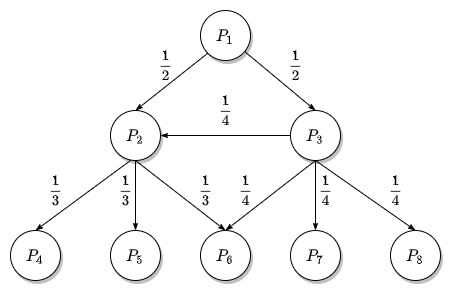
\includegraphics[width=0.5\textwidth]{./img/grafoprob}
\end{center}

Volvemos a considerar las mismas paginas web $P_1, P_2, \dots, P_n$ y $M$ la matriz de adyacencia del grafo, cuyas entradas $m_{ij}$ son $0$ y $1$. Llamamos $N_j$ al número de enlaces de la página $P_j$,  es decir al número de entradas de la columna $j$. Construimos una nueva matriz $M'$ a partir de la $M$ original sustituyendo cada $m_{ij}$ por
$$m'_{ij} = \frac{m_{ij}}{N_j} $$
La transformación sería la siguiente:

\begin{center}
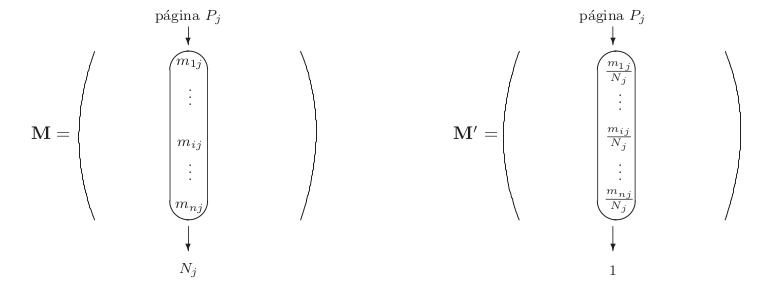
\includegraphics[width=0.9\textwidth]{./img/markov}
\end{center}

La nueva matriz $M'$ esta compuesta por números no negativos entre $0$ y $1$, a esta matriz así construida se le llama una matriz estocástica (o de Markov).

Con este modelo podemos conocer con que probabilidad estará el usuario en cada una de las páginas tras cada instante de tiempo, entendiendo instante de tiempo como transiciones o saltos. Por ejemplo, si el usuario parte de la página k-ésima $P_k$ para saber que probabilidad tiene de cambiar a cada uno de los posibles destinos solo tenemos que multiplicar la matriz $M'$ por el vector inicial. En este caso el vector inicial es un vector de ceros y un $1$ en la posición k-ésima, ya que sabemos que el usuario se encuentra en la página $P_k$ con una probabilidad 1.

Si multiplicamos $M'$ por el vector inicial, obtenemos:
$$\begin{pmatrix}
\cdots & \cdots & m'_{1k} & \cdots \\
\vdots & \ddots & \vdots & \vdots \\
\cdots & \cdtos & m'_{kk} & \cdots \\
\vdots & \vdots & \vdots & \ddots \\
\cdots & \cdots & m'_{nk} & \cdots \end{pmatrix} \begin{pmatrix}
0 \\
\vdots \\
1 \\
\vdots \\
0 \end{pmatrix} = \begin{pmatrix}
m'_{1k}\\
\vdots \\
m'_{kk} \\
\vdots \\
m'_{nk} \end{pmatrix}$$

Este vector resultante, cuyas entradas son o $0$ o $1/N_k$, describe con que probabilidad estará el usuario en cada una de las páginas tras una unidad de tiempo. Para saber con que probabilidad estará en cada uno de los posibles destinos dentro de dos unidades de tiempo solo debemos multiplicar el vector inicial por $(M')^2$, si lo queremos saber para dentro de tres unidades de tiempo lo multiplicaremos por $(M')^3$ y así sucesivamente.

La matriz $M'$ recibe el nombre de matriz de transición del sistema, ya que en cada entrada $m'_{ij}$ se refleja la probabilidad de pasar de la página $P_j$ a la página $P_i$. Y además las matrices que se corresponden con sus respectivas potencias también reflejan la probabilidad de pasar de $P_j$ a $P_i$ tras varios instantes de tiempo.

Sin embargo, podría ocurrir que alguna de las páginas no citaran a ninguna otra, es decir, que ese nodo del grafo no tuviera enlaces salientes. Esto se traduce en que en nuestra matriz $M'$ aparece una columna de ceros, por lo que esta matriz dejaría de ser estocástica y además el grafo del que partimos no estaría fuertemente conectado. Para solucionarlo se añade una probabilidad de transición a todos los vértices, es decir, añadimos la posibilidad de que el usuario se ``aburra'' y decida cambiar a otra página que no esté enlazada con la página en la que se encontraba. En términos matriciales se traduce en lo siguiente:

$$M'' = cM' + (1-c)\begin{pmatrix}
p_1 \\
\vdots \\
p_n \end{pmatrix} (1, \dots, 1)$$

\spanishdecimal{.}
Donde $p_1, \dots , p_n$ es una distribución de probabilidad y $c$ es un parámetro entre $0$ y $1$, el cual Google estima que se encuentra sobre $0,85$ \footnote{Valor extraido de \url{https://en.wikipedia.org/wiki/PageRank}}. La distribución de probabilidad a tomar puede ser una distribución uniforme que asigne una probabilidad de $p_i = 1/n$ \footnote{Donde $n$ es el número de Páginas web o documentos.} a cada página, aunque también se podría elegir otras, ponderando unas páginas más que otras consiguiendo así búsquedas más personalizadas.

\newpage

\section{Pseudocódigo}
En esta sección comentaremos la estructura del algoritmo. Para implementarlo hemos separado el algoritmo en dos funciones. La primera función (\verb|pagerank|) se encarga de construir la matriz de adyacencia del grafo formado por todos los archivos y sus citas, además normaliza esta matriz por columnas, como se indicó anteriormente, para conseguir la matriz de transición del sistema y por último se le añade la el parámetro $c$ y la distribución de probabilidad uniforme como se comenta anteriormente, consiguiendo la matriz $M''$. La segunda función (\verb|metodopotencias|) tiene como objetivo calcular el vector propio de nuestra matriz $M''$, para ello se utiliza el método de las potencias.

\begin{algorithm}[H]
  \KwData{Vector que contiene todos los nodos (v)}
  \KwResult{Vector de pesos del PageRank (pg)}
  m = construyeMatrizAdyaencia(v)\;
  \For{i \in len(v)}{
    \If{ sum(m.T[i]) != 0}{
      m.T[i] = m.T[i] / sum(m.T[i])\;
    }
  }
  N = m[0].size()\;
  m\_seg = (C * m + (1 - C)/N)\;
  pg = metodopotencias(m\_seg, 100)\;
  \Return pg
\caption{pagerank}
\end{algorithm}

\begin{algorithm}[H]
  \KwData{M'' (m); Número de interaciones (num\_iter)}
  \KwResult{Vector de pesos del PageRank (v)}

  N = m[0].size()\;
  v = random(N, 1)\;
  v = v / max(v)\;
  \For{i $\in$ num\_iter}{
    v = m \cdot v
  }
  \Return v

\caption{metodopotencias}
\end{algorithm}

En el primer pseudocódigo \verb|m.T| se refiere a la traspuesta de \verb|m| y la constante \verb|C| tiene un valor de $0.85$ fijado previamente.

\newpage

\section{Ejemplos}
Para ilustrar como funciona el algoritmo del PageRank vamos a mostrar unos ejemplos que van a ilustrar como la estructura de una página, lo que se traduce por una topología del grafo, afecta en el cálculo de los pesos\footnote{Recordemos que estos cambios pueden llevarse a cabo a diario, lo que implica un cambio de posicionamiento en el ranking.}. Comenzamos con el primer ejemplo \ref{ejemplo1}, en este nos damos cuenta de que tanto $P_4$ como $P_5$ tienen dos enlaces entrantes, sin embargo, queda primero en la clasificación $P_5$, después $P_1$ y en tercer lugar $P_4$. Esto se debe a que  una de los enlaces entrantes de $P_5$ es de $P_4$ una de las páginas con más enlaces. Recordemos que este algoritmo premia también si la página que cita es importante.

\underline{\textbf{Ejemplo 1}}
\begin{figure}[!ht]
  \begin{tabular}{*{2}{>{\centering\arraybackslash}b{\dimexpr0.5\linewidth-2\tabcolsep\relax}}}
  \centering
    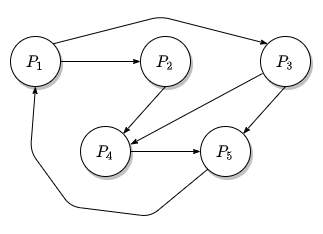
\includegraphics[scale=0.5]{./img/grafoej1}
    \caption{Grafo del ejemplo 1}
    \label{ejemplo1}

    &
      \renewcommand{\arraystretch}{1.3}
      \begin{tabular}{ccc}
         & Página & PageRank     \\ \hline
      1\textsuperscript{\underline{o}}} & $P_5$  & $0.26375504$ \\ \hline
      2\textsuperscript{\underline{o}}} & $P_1$  & $0.25419178$ \\ \hline
      3\textsuperscript{\underline{o}}} & $P_4$  & $0.20599017$ \\ \hline
      4\textsuperscript{\underline{o}}} & $P_2$  & $0.13803151$ \\ \hline
      5\textsuperscript{\underline{o}}} & $P_3$  & $0.13803151$ \\ \hline
      \end{tabular}\captionof{table}{Clasificación del ejemplo 1}
  \end{tabular}
\end{figure}

Para el ejemplo 2 le añadimos al ejemplo anterior dos páginas nuevas que también citan a $P_4$ como puede verse en \ref{ejemplo2}, sin embargo, esto no hace que $P_4$ se coloque en primera posición. Queda reflejado que el algoritmo da más puntuación a que la página tenga un enlace de una página importante que a una página con muchos enlaces, como puede verse en la tabla \ref{tablaejemplo2}

\underline{\textbf{Ejemplo 2}}

\begin{figure}[!ht]
  \begin{tabular}{*{2}{>{\centering\arraybackslash}b{\dimexpr0.5\linewidth-2\tabcolsep\relax}}}
  \centering
    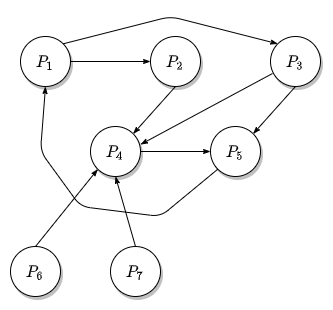
\includegraphics[scale=0.5]{./img/grafoej2}
    \caption{Grafo del ejemplo 2}
    \label{ejemplo2}
    &
      \renewcommand{\arraystretch}{1.3}
      \begin{tabular}{ccc}
        & Página & PageRank     \\ \hline
      1\textsuperscript{\underline{o}}} & $P_5$  & $0.2564552$  \\ \hline
      2\textsuperscript{\underline{o}}} & $P_1$  & $0.2394155$  \\ \hline
      3\textsuperscript{\underline{o}}} & $P_4$  & $0.21491184$ \\ \hline
      4\textsuperscript{\underline{o}}} & $P_2$  & $0.12318016$ \\ \hline
      5\textsuperscript{\underline{o}}} & $P_3$  & $0.12318016$ \\ \hline
      6\textsuperscript{\underline{o}}} & $P_7$  & $0.02142857$ \\ \hline
      7\textsuperscript{\underline{o}}} & $P_6$  & $0.02142857$ \\ \hline
      \end{tabular}\captionof{table}{Clasificación del ejemplo 2}\label{tablaejemplo2}
    \end{tabular}
\end{figure}

\newpage

Para el ejemplo 3, ver figura \ref{ejemplo3}, cambiamos la estrategia. Partimos del ejemplo 1 y en vez de añadir citas desde páginas nuevas hasta $P_4$ le añadimos una cita desde una de las páginas del grafo inicial, $P_1$, y observamos que tampoco conseguimos quitar a $P_5$ del primer puesto aunque la $P_4$ tenga más enlaces entrantes.

\underline{\textbf{Ejemplo 3}}

\begin{figure}[!ht]
  \begin{tabular}{*{2}{>{\centering\arraybackslash}b{\dimexpr0.5\linewidth-2\tabcolsep\relax}}}
  \centering
    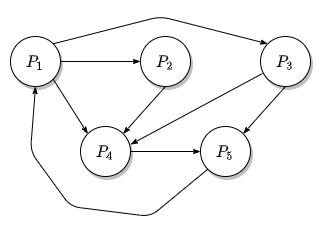
\includegraphics[scale=0.5]{./img/grafoej3}
    \caption{Grafo del ejemplo 3}
    \label{ejemplo3}
    &
      \renewcommand{\arraystretch}{1.3}
      \begin{tabular}{ccc}
        & Página & PageRank     \\ \hline
      1\textsuperscript{\underline{o}}} & $P_5$  & $0.27969961$ \\ \hline
      2\textsuperscript{\underline{o}}} & $P_1$  & $0.26774467$ \\ \hline
      3\textsuperscript{\underline{o}}} & $P_4$  & $0.24083375$ \\ \hline
      4\textsuperscript{\underline{o}}} & $P_2$  & $0.10586099$ \\ \hline
      5\textsuperscript{\underline{o}}} & $P_3$  & $0.10586099$ \\ \hline
      \end{tabular}\captionof{table}{Clasificación del ejemplo 3}
    \end{tabular}
\end{figure}

En el ejemplo anterior se comprueba la importancia del enlace saliente de $P_4$ capaz de colocar a una página en el primer puesto del ranking. De hecho si cambiamos este enlace y ponemos que salga de $P_4$ y llegue a $P_1$ convertimos a $P_1$ en la primera del ranking.

\underline{\textbf{Ejemplo 4}}

\begin{figure}[!ht]
  \begin{tabular}{*{2}{>{\centering\arraybackslash}b{\dimexpr0.5\linewidth-2\tabcolsep\relax}}}
  \centering
    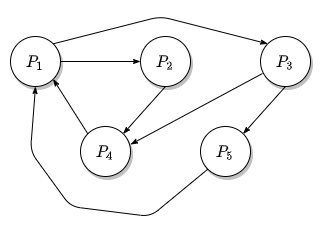
\includegraphics[scale=0.5]{./img/grafoej4}
    \caption{Grafo del ejemplo 4}
    &
      \renewcommand{\arraystretch}{1.3}
      \begin{tabular}{ccc}
        & Página & PageRank     \\ \hline
      1\textsuperscript{\underline{o}}} & $P_1$  & $0.32225461$ \\ \hline
      2\textsuperscript{\underline{o}}} & $P_4$  & $0.24287173$ \\ \hline
      3\textsuperscript{\underline{o}}} & $P_2$  & $0.16695821$ \\ \hline
      4\textsuperscript{\underline{o}}} & $P_3$  & $0.16695821$ \\ \hline
      5\textsuperscript{\underline{o}}} & $P_5$  & $0.10095724$ \\ \hline
      \end{tabular}\captionof{table}{Clasificación del ejemplo 4}
    \end{tabular}
\end{figure}

\newpage

Para conseguir que $P_4$, la página con más enlaces entrantes, se posicione la primera de la clasificación, partiendo del grafo del ejemplo 1 se eliminan los enlaces salientes de $P_4$, como puede verse en \ref{ejemplo5}.

\underline{\textbf{Ejemplo 5}}

\begin{figure}[!ht]
  \begin{tabular}{*{2}{>{\centering\arraybackslash}b{\dimexpr0.5\linewidth-2\tabcolsep\relax}}}
  \centering
    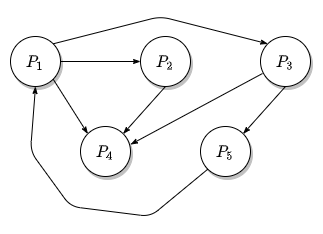
\includegraphics[scale=0.5]{./img/grafoej5}
    \caption{Grafo del ejemplo 5}
    \label{ejemplo5}
    &
      \renewcommand{\arraystretch}{1.3}
      \begin{tabular}{ccc}
        & Página & PageRank         \\ \hline
      1\textsuperscript{\underline{o}}} & $P_4$  & $2.79048247e-13$ \\ \hline
      2\textsuperscript{\underline{o}}} & $P_1$  & $2.47850051e-13$ \\ \hline
      3\textsuperscript{\underline{o}}} & $P_5$  & $1.86281319e-13$ \\ \hline
      4\textsuperscript{\underline{o}}} & $P_2$  & $1.31449230e-13$ \\ \hline
      5\textsuperscript{\underline{o}}} & $P_3$  & $1.31449230e-13$ \\ \hline
      \end{tabular}\captionof{table}{Clasificación del ejemplo 5}
    \end{tabular}
\end{figure}

Con los ejemplos mostrados podemos observar que para el algoritmo puntúa más un enlace que sale de una página ``importante'' que muchos enlaces de páginas ``poco importantes''. En el siguiente ejemplo, ejemplo 6 \ref{ejemplo6}, vemos que la página que más enlaces tiene es $P_3$ y la segunda $P_4$. Siguiendo el razonamiento anterior $P_3$ sería una página ``importante'' y su enlace valdría mucho, tanto que es capaz de colocar a cualquier página en primera posición. En este caso $P_3$ cita a $P_5$ convirtiéndola en una página ``importante'' y colocandola en primer lugar en la clasificación. Sin embargo, en este ejemplo añadimos un enlace desde $P_5$, página importante, a $P_3$ que también es importante, el resultado es un ajustado desempate (& $1.48851482e-06$ frente a $1.37701780e-06$) en el que resulta ganador $P_5$.

\underline{\textbf{Ejemplo 6}}

\begin{figure}[!ht]
  \begin{tabular}{*{2}{>{\centering\arraybackslash}b{\dimexpr0.5\linewidth-2\tabcolsep\relax}}}
  \centering
    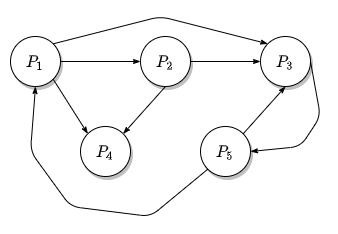
\includegraphics[scale=0.5]{./img/grafoej6}
    \caption{Grafo del ejemplo 6}
    \label{ejemplo6}
    &
      \renewcommand{\arraystretch}{1.3}
      \begin{tabular}{ccc}
        & Página & PageRank         \\ \hline
      1\textsuperscript{\underline{o}}} & $P_5$  & $1.48851482e-06$ \\ \hline
      2\textsuperscript{\underline{o}}} & $P_3$  & $1.37701780e-06$ \\ \hline
      3\textsuperscript{\underline{o}}} & $P_1$  & $8.80201594e-07$ \\ \hline
      4\textsuperscript{\underline{o}}} & $P_4$  & $6.61515329e-07$ \\ \hline
      5\textsuperscript{\underline{o}}} & $P_2$  & $4.46763904e-07$ \\ \hline
      \end{tabular}\captionof{table}{Clasificación del ejemplo 6}
    \end{tabular}
\end{figure}

Por último, nos preguntamos si las dos páginas tienen el mismo número de enlaces entrantes $P_3$ y $P_4$, partiendo de una situación de ``empate'' y una de ellas no tiene enlaces salientes $P_4$. Como puede verse en figura~\ref{ejemplo7} y tabla~\ref{tablaejemplo7}. Observamos que los valores son muy ajustados, aunque $P_5$ se sitúa en primer lugar del \textit{ranking} (gracias al enlace desde $P_3$), en segundo puesto quedaría $P_3$ y en tercer lugar $P_4$. Por lo que una página sino dispone de enlaces salientes tan solo puede subir en el \textit{ranking} si tiene más enlaces entrantes que las demás páginas.

\underline{\textbf{Ejemplo 7}}

\begin{figure}[!ht]
  \begin{tabular}{*{2}{>{\centering\arraybackslash}b{\dimexpr0.5\linewidth-2\tabcolsep\relax}}}
  \centering
    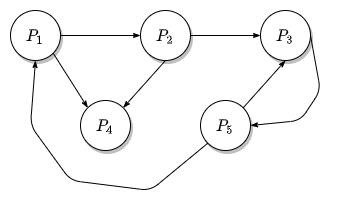
\includegraphics[scale=0.5]{./img/grafoej7}
    \caption{Grafo del ejemplo 7}
    \label{ejemplo7}
    &
      \renewcommand{\arraystretch}{1.3}
      \begin{tabular}{ccc}
        & Página & PageRank         \\ \hline
      1\textsuperscript{\underline{o}}} & $P_5$  & $7.66066766e-09$ \\ \hline
      2\textsuperscript{\underline{o}}} & $P_3$  & $6.60140578e-09$ \\ \hline
      3\textsuperscript{\underline{o}}} & $P_4$  & $5.18659092e-09$ \\ \hline
      4\textsuperscript{\underline{o}}} & $P_1$  & $4.86047008e-09$ \\ \hline
      5\textsuperscript{\underline{o}}} & $P_2$  & $3.44565523e-09$ \\ \hline
      \end{tabular}\captionof{table}{Clasificación del ejemplo 7}\label{tablaejemplo7}
    \end{tabular}
\end{figure}

\newpage

\section{Conjunto de datos}
\label{Base de datos}
Para implementar el algoritmo de PageRank se ha utilizado el conjunto de datos \textbf{PMSC-UGR} con $26759991$ artículos. Este conjunto de datos basado en artículos científicos de MEDLINE/PubMed  pero también utilizando SCopus herramienta de Elsevier. Por razones de eficiencia se ha tenido que procesar el conjunto de datos para poder aplicar el cálculo de PageRank, los datos de la colección inicial se redujeron a 3000 documentos, todos relacionados entre ellos, los cuales constan de una 26000 palabras. Esta división ha sido necesaria puesto que en el intento de implementar el algoritmo con todos los artículos la matriz creada alcanzaba una dimensión muy grande impidiendo que el ordenador utilizado pudiera operar con ella, lo que habría requerido técnicas de paralelización de tareas para hacerlas más escalable, sin embargo esto quedaba fuera de los objetivos iniciales del proyecto. Estos 3000 documentos tomarán el papel de las páginas, ya que con las citas se puede construir un grafo dirigido al que aplicar el PageRank. En PSMC-UGR se ha hecho el esfuerzo de quitar las ambigüedades de los nombres de autores, para ello se ha establecido el ORCID, un número que identifica a cada autor de manera unívoca. Cada archivo esta estructurado de la siguiente forma:
\begin{itemize}
\item \textit{PubMedID}. Es un identificador único del articulo proporcionado por PubMed.
\item \textit{Journal}. Es el nombre de la revista donde el artículo ha sido publicado.
\item \textit{ArticleTitle}. Es el título completo del artículo en inglés.
\item \textit{Abstract}. Resumen del artículo.
\item \textit{AuthorList}. Contiene información sobre los autores del artículo. Por cada uno podemos encontrar:
\begin{itemize}
\item \textit{LastName}. Contiene el apellido o el nombre único utilizado.
\item \textit{ForeName}. Contiene el resto del nombre.
\item \textit{Identifier}. Es un identificador único asociado con el nombre (ORCID).
\end{itemize}
\item \textit{MeshHeadingList}. Es un vocabulario controlado por NLM, encabezados de temas médicos (Mesh). Se utiliza para caracterizar el contenido del artículo utilizando descriptores de ese tesauro.
\item \textit{KeywordList}. Contiene términos controlados en palabras clave que también describen el contenido del artículo.
\end{itemize}

A estos datos se añaden las citas, el $66.78 \%$ de los artículos tienen alguna cita. La media de citas por artículo es de 7 y el total de citas es $3593931$. El número de citas por artículo sigue una típica distribución \textit{ley de potencia} donde pocos artículos tienen muchas citas y muchos artículos tienen pocas citas. Por ejemplo, hay $116365$ artículos que tienen solo una cita y hay un artículo que tiene 713 citas.

Además este conjunto de datos ha sido procesado añadiendo las referencias de cada artículo, es decir, cada artículo conoce quien lo ha citado. Este dato no se utiliza en el algoritmo ya que por lo general no se suele conocer, cada artículo solo sabe que artículos ha citado y no llega a conocer los otro artículos que lo han citado.

\newpage

\section{Modelos de Recuperación de Información}
La Recuperación de Información (RI) busca acceder a contenidos mediante modelos que posteriormente se diseñan e implementan. Su finalidad es estimar la relevancia de los datos a la necesidad de información de un usuario la cual se expresa en una consulta.
En nuestro caso, buscamos acceder a la información de nuestro conjunto de datos formada por una selección de documentos. A través de una consulta buscamos mostrar información relevante para el usuario que la ha introducido.

Según \cite{ri} podemos definir un modelo de RI como una cuádrupla $[D,Q,F,R(q_i,f_j)]$, donde:
\begin{itemize}
\item $D$ es el conjunto de representaciones de los documentos.
\item $Q$ es el conjunto de representaciones de necesidades de información de los usuarios.
\item $F$ es le conjunto de representaciones de las relaciones entre documentos y consultas.
\item $R(q_i,d_j)$ es la función de selección y ordenación que permite entregar al usuario unos documentos (ordenados o no) en respuesta a una consulta.
\end{itemize}

\subsection{Modelo booleano}
Este modelo se basa en la teoría de conjuntos y la lógica booleana, como ya comentamos anteriormente solo tiene en cuenta la presencia de alguna de las palabras o términos de la consulta en el documento. En él, no se tiene en cuenta ni la frecuencia, ni la importancia del término en el documento o en la colección.

Según el libro \cite{ri} definimos el conjunto de todos los términos de la colección de documentos como $V = \{t_1, t_2, \dots, t_M \}$ y el conjunto de todos los documentos de la colección como $D = \{ d_1, d_2, \dots, d_N \}$. Cada documento $d_j$ se va a representar como un subconjunto de $V$ donde se encuentran los términos que aparecen en ese documento. Por otro lado, dispondremos de una estructura adicional, un índice invertido, cuya entrada es el termino, esto es, para cada término $t_i$ se define el conjunto $T_i$ formado por los documentos que contienen el término $t_i$ por lo tanto $T_i$ es un subconjunto de $D$.

En este modelo se representan las consultas mediante expresiones booleanas en las cuales se utilizan además de los términos, los operadores booleanos AND, OR y NOT. Como se detallará posteriormente se ha diseñado una interfaz para la introducción de consultas con las sintaxis de los operadores lógicos estándares. A continuación se muestra la forma de explotar el modelo con unas consultas de ejemplo.

El operador AND es un operador binario (necesita dos términos) que indica que se desea buscar los documentos que contentan ambos términos. Por ejemplo, si el usuario escribe ``perro AND gato'' está buscando los documentos que contienen tanto la palabra ``perro'' como la palabra ``gato''. Formalmente lo que indica es que se realiza la intersección de dos conjuntos, el conjunto formado por los documentos que contienen la palabra ``perro'' ($T_1$) y los que tienen la palabra ``gato'' ($T_2$).

Si por ejemplo tuvieramos los siguientes cuatro documentos:
\begin{itemize}
\item $d_1 = $ \{gato, gato, gato, tortuga, pez\}
\item $d_2 = $ \{perro, caballo\}
\item $d_3 = $ \{gato, perro, águila\}
\item $d_4 = $ \{pez, tortuga, tortuga\}
\end{itemize}
Entonces la consulta obtendría el siguiente resultado:
$$\textrm{perro AND gato } = T_1 \cap T_2 = \{d_2, d_3\} \cap \{d_1, d_3\} = \{d_3\}$$

El operador OR también binario, indica que se desea buscar los documentos que contengan un término o el otro. Siguiendo el ejemplo anterior si el usuario escribe ``perro OR gato'' está buscando los documentos que contengan la palabra ``perro'', o que contengan la palabra ``gato'' o que contenga ambas. Formalmente lo podemos representar como la unión de los conjuntos formados por los documentos que contienen la palabra ``perro'' ($T_1$) y los que tienen la palabra ``gato'' ($T_2$).
$$\textrm{perro OR gato } = T_1 \cup T_2 = \{d_2, d_3\} \cup \{d_1, d_3\} = \{d_1, d_2, d_3\}$$

Por último, el operador NOT es un operador unario (solo necesita un término) e indica que se desean buscar todos los documentos que no contengan ese término. Este operador se suele combinar con los dos anteriores ya que hace referencia a un conjunto de documentos muy amplio. Este operador se puede representar como la diferencia de conjuntos, el primero conjunto formado por todos los documentos $D$ y el segundo conjunto formado por las palabras que contienen el término. Por ejemplo:
$$\textrm{perro AND NOT gato } = T_1 \cap T_2 = \{d_2, d_3\} \cap \{d_2, d_4\} = \{d_2\}$$
$$\textrm{perro OR NOT gato } = T_1 \cup T_2 = \{d_2, d_3\} \cup \{d_2, d_4\} = \{d_2, d_3, d_4\}$$

Estos operadores se pueden anidar formando consultas más complejas. Por ejemplo, si llamamos, al igual que antes, $T_1$ a los documentos que tienen la palabra ``perro'', $T_2$ a los que tienen la palabra ``gato'' y llamamos ahora $T_3$ a los documentos que contienen la palabra ``tortuga'', la siguiente consulta tendría el resultado:
$$(\textrm{tortuga OR gato}) \textrm{ AND perro } = (T_3 \cup T_2) \cap T_1 = (\{d_1, d_4\} \cup \{d_1, d_3\}) \cap \{d_2, d_3\} =$$ $$= \{d_1, d_3, d_4\} \cap \{d_2 , d_3\} = \{d_3\} $$

El orden de los documento del resultado vendría dado por el PageRank, calculado previamente.

Una de las ventajas de este modelo es su sencillez de implementación, además posee una gran flexibilidad a la hora de realizar las distintas consultas gracias al uso de los operadores lógicos.

Por otro lado, solo se tiene en cuenta la presencia del término de la consulta en cada uno de los documentos. Esto puede ser un error ya que hay términos que cobran más importancia que otros y cuya aparición en el documento debería aumentar la relevancia de éste. Por otro lado, tampoco se tiene en cuenta la frecuencia de cada término en los documentos, no es lo mismo que la palabra aparezca solo una vez que aparezca más de una. Estos inconvenientes se resuelven en el siguiente modelo.

\subsection{Modelo vectorial}
En este modelo se construye un vector por cada documento y consulta en donde se reflejan los términos de cada una de ellas. Es decir, se crea un espacio vectorial de tamaño el número de términos de la colección de documentos.

Según el libro \cite{ri}, definimos $V$ y $D$ al igual que en el modelo anterior y definimos un documento $d_j$ como un vector de términos $d_j = (w_{1,j}, w_{2,j}, \dots, w_{M,j})$ donde $w_{i,j}$ indica el peso del término $i$ en el documento $j$. Este peso valdrá cero si el término no está presente en el documento y en caso de que aparezca tendrá peso positivo.

Con los datos anteriores creamos una matriz de pesos en donde representamos por filas todos los términos y por columnas todos los documentos, quedando la siguiente estructura:

\begin{center}
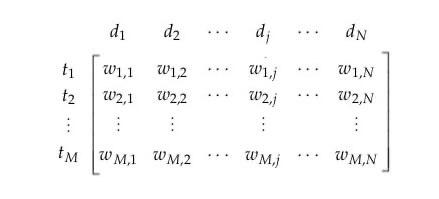
\includegraphics[scale=0.6]{./img/matrizpesos}
\end{center}

Este modelo se basa en dos conceptos fundamentales:
\begin{itemize}
\item Esquema de pesos.
\item Similitud entre dos vectores de términos (por ejemplo, entre un documento y una consulta).
\end{itemize}
Para definir una medida de adecuación de una consulta $q$ con cada documento $d$ se habla de similitud. La similitud entre los vectores de términos $q$ y $d$ se va a calcular mediante la distancia coseno que se define según el libro \cite{ri} como:
$$sim(q,d) = cos(\alpha) = \frac{\sum_{i = 1}^M w_{i,q} \cdot w_{i,d}}{\sqrt{\sum_{i = 1}^M w_{i,d}^2} \cdot \sqrt{\sum_{i = 1}^M w_{i,q}^2}} = \frac{q}{|q|} \cdot \frac{d}{|d|} $$

Por otro lado, a la hora de calcular el peso de un término en cada documento debemos tener en cuenta dos conceptos:
\begin{itemize}
\item La frecuencia del término en el documento ya que cuanto más se repita más importancia tendrá este término en el documento.
\item La especificidad del término en el documento; es decir, cuanto menos usual sea la palabra dentro de la colección de documentos más peso tendrá esta al considerarse relevante su aparición.
\end{itemize}
Utilizaremos el modelo \textit{tf.idf}, mencionado en el libro \cite{ri},  formado por dos componentes que representan los conceptos explicados anteriormente:
\begin{itemize}
\item \textit{Term frequency} (tf): indica la frecuencia del término en el documento.
\item \textit{Inverse document frequency} (idf): número de documentos en donde aparece referenciado el término pero a la inversa. Se da mayor peso a loa términos que se encuentran en un número menor de documentos.
\end{itemize}

Por lo tanto, calcularemos el peso de un término de la siguiente forma:
$$w_{i,j} = tf_{i,j} \cdot idf_i = tf_{i,j} \cdot \log \left(\frac{N}{n_i} \right) $$
Donde $tf_{i,j}$ es la frecuencia del término $i$ en el documento $j$, $N$ es el número de documento que tiene la colección y $n_i$ es el número de documentos en donde aparece el término $i$.

Tras calcular estos pesos se normaliza cada vector $d_j$, es decir, dividimos el vector por su longitud:
$$d_j = \frac{d_j}{|d_j|} \textrm{ donde } |v| = \sqrt{\sum_{i = 1}^M v_i^2} $$

Por último, el procedimiento consistirá en calcular los pesos de la consulta $q$ y calcular la similitud de la consulta con cada documento de la colección. Tras estas operaciones se obtiene un vector de relevancia donde queda reflejada la similitud de cada documento a la consulta, estas similitudes son multiplicadas por el vector del PageRank para obtener el nuevo orden.

Retomamos el anterior ejemplo, donde el conjunto $D$ estaba formado por los documentos:
\begin{itemize}
\item $d_1 = $ \{gato, gato, gato, tortuga, pez\}
\item $d_2 = $ \{perro, caballo\}
\item $d_3 = $ \{gato, perro, águila\}
\item $d_4 = $ \{pez, tortuga, tortuga\}
\end{itemize}
Por tanto, los términos son $V=$\{gato, tortuga, pez, perro, caballo, águila\}, y supongamos que la consulta es $q =$\{gato, tortuga\}.
La matriz $tf$ sería la siguiente:
\begin{table}[H]
\centering
\begin{tabular}{|c|c|c|c|c|c|}
\hline
$tf$    & $d_1$ & $d_2$ & $d_3$ & $d_4$ & $q$ \\ \hline
gato    & 3     & 0     & 1     & 0     & 1   \\ \hline
tortuga & 1     & 0     & 1     & 2     & 1   \\ \hline
pez     & 1     & 0     & 0     & 1     & 0   \\ \hline
perro   & 0     & 1     & 1     & 0     & 0   \\ \hline
caballo & 0     & 1     & 0     & 0     & 0   \\ \hline
águila  & 0     & 0     & 1     & 0     & 0   \\ \hline
\end{tabular}
\end{table}
Mostramos a continuación la matriz $w$ ya normalizada:
\begin{table}[H]
\centering
\begin{tabular}{|c|c|c|c|c|c|}
\hline
$tf$    & $d_1$ & $d_2$ & $d_3$ & $d_4$ & $q$  \\ \hline
gato    & 0.94  & 0     & 0.40  & 0     & 0.92 \\ \hline
tortuga & 0.13  & 0     & 0.17  & 0.64  & 0.38 \\ \hline
pez     & 0.31  & 0     & 0     & 0.77  & 0    \\ \hline
perro   & 0     & 0.45  & 0.40  & 0     & 0    \\ \hline
caballo & 0     & 0.89  & 0     & 0     & 0    \\ \hline
águila  & 0     & 0     & 0.81  & 0     & 0    \\ \hline
\end{tabular}
\end{table}
El resultado de calcular la similitud de la consulta entre todos los documentos se muestra en la siguiente tabla:
\begin{table}[H]
\centering
\begin{tabular}{|c|c|c|c|c|}
\hline
sim & $d_1$ & $d_2$ & $d_3$ & $d_4$ \\ \hline
$q$ & 0.92  & 0     & 0.43  & 0.24  \\ \hline
\end{tabular}
\end{table}
Por último, se multiplicaría este vector con el vector del PageRank componente a componente. Para este modelo no estarán disponibles los operadores lógicos en la interfaz, ya que carece de sentido.

\subsection{Técnicas de modificación de la consulta}
Hasta el momento, ya sea utilizando el modelo booleano o el modelo vectorial, una misma consulta realizada por distintos usuarios obtiene el mismo conjunto de documentos relevantes o el mismo \textit{ranking} determinado por los términos y el PageRank. Sin embargo, nos planetamos la posibilidad de alterar estos resultados en función de quién realizará la consulta, tratando de personalizar las consultas en función de su perfil o interés habitual. Se trataba de explorar cómo se puede alterar este \textit{ranking}. Google cuenta con log, consultas y documentos explorados con anterioridad por un usuario para realizar esta alteración personalizada del \textit{ranking}. Con los datos disponibles de la colección determinamos utilizar un perfil de usuario formado por aquellos términos de los documentos que le son más relevantes, en el caso ideal por lo documentos redactados por ellos mismos. Con este propósito decidimos explorar la realimentación de consultas la cual busca expandir la consulta utilizando los primeros documentos más relevantes para ello.

Una de las mayores ventajas de esta técnica es que se trata de un proceso automático, no necesita de la intervención del usuario. Sin embargo, la efectividad de la técnica depende de la bondad del primer resultado, si la consulta devuelve un resultado donde los documentos son relevantes la extensión de la consulta conseguirá recuperar los documentos más relevantes, pero si por el contrario la primera recuperación no es buena aparecerán en la consulta expandida términos relacionados con ella por lo que esta será menos relevante aún para el usuario.

El objetivo de esta técnica consiste en conseguir una consulta expandida $q'$ a partir de una consulta $q$, para ello se utiliza la fórmula de Rocchio extraída del libro \cite{ri}:
$$q' = \alpha q + \frac{\beta}{D_r} \sum_{d_j \in D_r} d_j - \frac{\gamma}{D_{nr}} \sum_{d_j \in D_{nr}} d_j $$
Donde $D_{r}$ es el conjunto de documentos que previamente se han fijado como relevantes para el usuario y $D_{nr}$ son los documentos no relevantes. Mientras que $\alpha$, $\beta$ y $\gamma$ son parámetros que hay que fijar. Usualmente se le da valores $\alpha = 1$, $\beta = 0.75$ y $\gamma = 0$, ya que no buscamos ampliar la consulta con documentos no relevantes.

Tras calcular la nueva consulta $q'$ se vuelve a calcular la similitud entre esta y los documentos, obteniendo un vector que refleja la similitud de la nueva consulta $q'$ y los documentos, este vector se multiplica por el vector del PageRank para obtener el nuevo orden.

Reutilizamos el ejemplo anterior donde la matriz de pesos era:
\begin{table}[H]
\centering
\begin{tabular}{|c|c|c|c|c|c|}
\hline
$tf$    & $d_1$ & $d_2$ & $d_3$ & $d_4$ & $q$  \\ \hline
gato    & 0.94  & 0     & 0.40  & 0     & 0.92 \\ \hline
tortuga & 0.13  & 0     & 0.17  & 0.64  & 0.38 \\ \hline
pez     & 0.31  & 0     & 0     & 0.77  & 0    \\ \hline
perro   & 0     & 0.45  & 0.40  & 0     & 0    \\ \hline
caballo & 0     & 0.89  & 0     & 0     & 0    \\ \hline
águila  & 0     & 0     & 0.81  & 0     & 0    \\ \hline
\end{tabular}
\end{table}
Aplicamos la ecuación de Rocchio con parámetros $\alpha = 1$, $\beta = 0.75$ y $\gamma = 0$ suponiendo que los documentos que tienen interés para el usuario son, por ejemplo $d_1$ y $d_3$:
\begin{table}[H]
\centering
\begin{tabular}{|c|c|c|c|c|}
\hline
 & $1 \cdot q$ & $(0.75/2) \cdot d_1$ & $(0.75/2) \cdot d_3$ & Rocchio \\ \hline
gato    & 0.92        & 0.35                 & 0.15                 & 1.42 \\ \hline
tortuga & 0.38        & 0.05                 & 0.06                 & 0.49 \\ \hline
pez     & 0           & 0.12                 & 0                    & 0.12 \\ \hline
perro   & 0           & 0                    & 0.15                 & 0.15 \\ \hline
caballo & 0           & 0                    & 0                    & 0    \\ \hline
águila  & 0           & 0                    & 0.30                 & 0.30 \\ \hline
\end{tabular}
\end{table}
A continuación nos quedaríamos con los 10 ó 15 términos con mayor valor, pero como en este caso solo tenemos 6 términos, nos quedaremos con los 4 mayores, por lo tanto $q'$ tendría el siguiente valor:
\begin{table}[H]
\centering
\begin{tabular}{|c|c|}
\hline
        & $q'$  \\ \hline
gato    & 1.42 \\ \hline
tortuga & 0.49 \\ \hline
pez     & 0    \\ \hline
perro   & 0.15 \\ \hline
caballo & 0    \\ \hline
águila  & 0.30 \\ \hline
\end{tabular}
\end{table}
La similitud de la nueva consulta $q'$ es:
\begin{table}[H]
\centering
\begin{tabular}{|c|c|c|c|c|}
\hline
sim  & $d_1$ & $d_2$ & $d_3$ & $d_4$ \\ \hline
$q'$ & 0.91  & 0.04  & 0.62  & 0.20  \\ \hline
\end{tabular}
\end{table}
Vemos que al contrario que en la anterior consulta el documento $d_2$ obtiene algo de relevancia ($0.04$) esto es debido a que uno de los documentos importantes para el usuario es el $d_3$ y ambos contienen el término ``perro''.
Por último, al igual que en el método anterior este vector de relevancias se multiplicará término a término por el vector de PageRank.

\newpage

\section{Interfaz gráfica}
Para mostrar mejor los resultados del buscador y mejorar la comunicación entre el usuario y el sistema se ha desarrollado una interfaz gráfica cuya apariencia es la siguiente:

\begin{figure}[H]
\centering
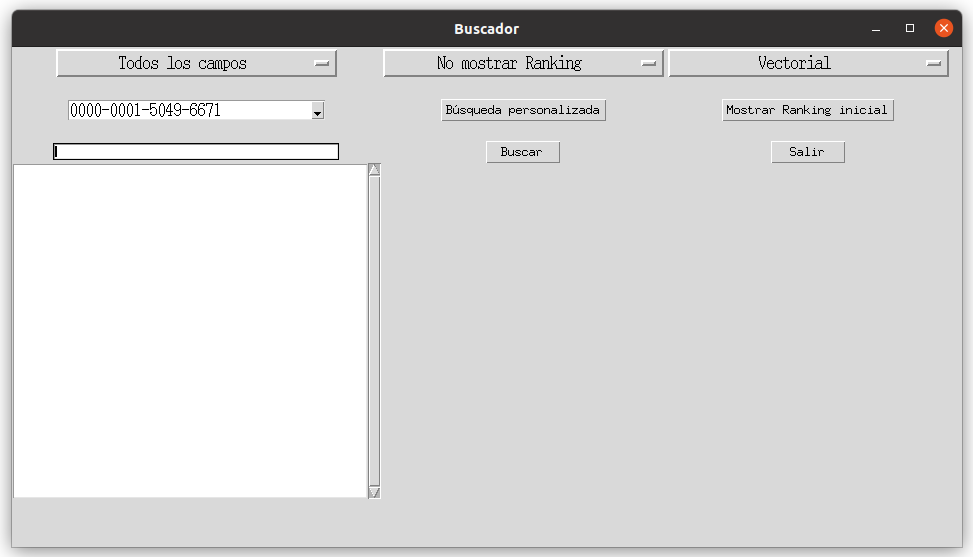
\includegraphics[width=1.0\textwidth]{interfaz}
\caption{Interfaz gráfica del buscador.}
\end{figure}

En el desplegable situado en la parte superior a la izquierda se puede seleccionar el modelo que deseamos utilizar (Vectorial o Booleano).

\begin{figure}[H]
\centering
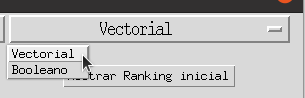
\includegraphics[width=0.8\textwidth]{modelo}
\caption{Desplegable para seleccionar el modelo.}
\end{figure}

Como ya explicamos anteriormente dependiendo del modelo las consultas se realizan de forma distinta:
\begin{itemize}
\item \textbf{\underline{Modelo booleano}}. En este modelo se puede elegir en que parte del documento se quiere realizar la búsqueda: título, abstract, palabras clave o todos las partes. Este dato se indica en el desplegable situado en la parte superior izquierda.

\begin{figure}[H]
\centering
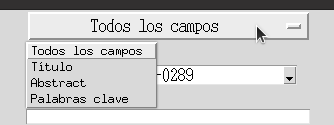
\includegraphics[width=0.8\textwidth]{sitio}
\caption{Desplegable para seleccionar la parte del documento en donde se desea realizar la búsqueda.}
\end{figure}

Una vez seleccionado en que parte del documento deseamos realizar la búsqueda, introducimos la consulta con las correspondientes expresiones lógicas y pulsamos en el botón ``Buscar''. Por ejemplo, introducimos la consulta ``cognitive AND papers''.

\begin{figure}[H]
\centering

\includegraphics[width=0.8\textwidth]{consultabool}
\caption{Celda donde se introduce la consulta y botón que dispara la búsqueda.}
\end{figure}
El resultado de la búsqueda se mostrará en el espacio situado justo debajo de la celda donde se introduce la consulta.

\begin{figure}[H]
\centering
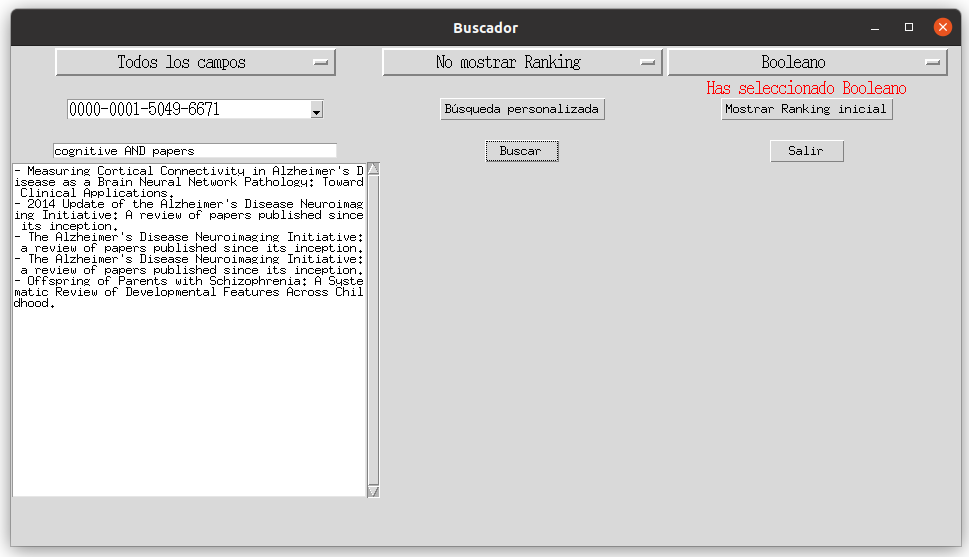
\includegraphics[width=1.0\textwidth]{bool}
\caption{Resultado de la búsqueda en el modelo booleano.}
\end{figure}

\item \textbf{\underline{Modelo vectorial}}. En este modelo podemos elegir entre realizar una consulta normal basada únicamente en términos o una consulta personalizada. Para realizar una consulta normal solo hay que introducir la consulta en la celda y pulsar el botón ``buscar'' (en este modelo no se utilizan esquemas lógicos). Por ejemplo, podemos buscar las palabras ``extension network''.

\begin{figure}[H]
\centering

\includegraphics[width=0.8\textwidth]{consultavec}
\caption{Celda donde se introduce la consulta y botón que dispara la búsqueda.}
\end{figure}
\end{itemize}

Cuyo resultado sería:

\begin{figure}[H]
\centering
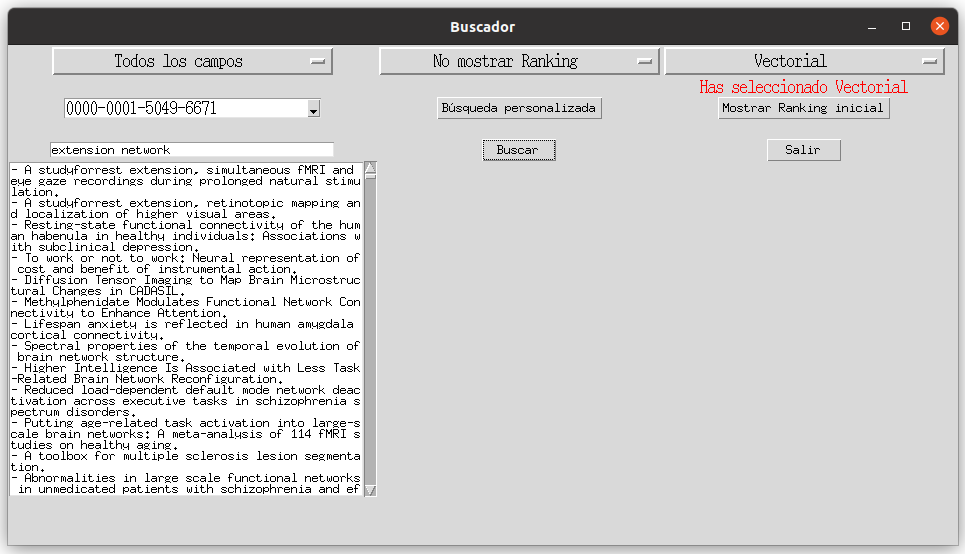
\includegraphics[width=1.0\textwidth]{vec}
\caption{Resultado de la búsqueda en el modelo vectorial (búsqueda normal).}
\end{figure}
Para realizar una búsqueda personalizada, primero debemos elegir el usuario que la realiza. Como ya se ha comentado anteriormente los usuarios son los propios autores de los documentos, que han sido previamente identificados por un ORCID. Para elegir que usuario realiza la consulta se utiliza el desplegable situado justo encima de la celda de la consulta y se selecciona uno de los ORCID.
\begin{figure}[H]
\centering
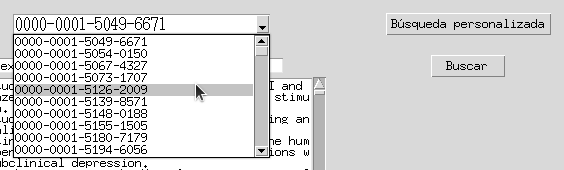
\includegraphics[width=0.8\textwidth]{autores}
\caption{Desplegable para elegir el ORCID del autor que realiza la búsqueda.}
\end{figure}

Por ejemplo, seleccionamos el autor $0000-0001-6983-0641$, introducimos la consulta de nuevo en la celda y pulsamos el botón ``Búsqueda personalizada'' para disparar la búsqueda. Por ejemplo, realizamos la consulta ``activation scale''.

\begin{figure}[H]
\centering
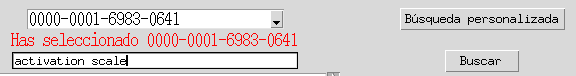
\includegraphics[width=0.8\textwidth]{consultaper}
\caption{Celda donde se introduce la consulta y botón que dispara la búsqueda.}
\end{figure}
\end{itemize}
Cuyo resultado es el siguiente:
\begin{figure}[H]
\centering
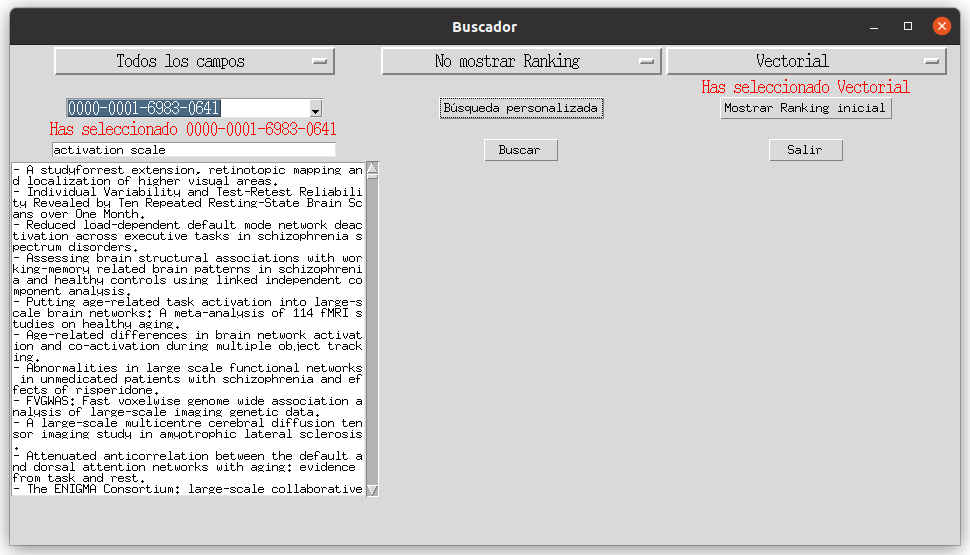
\includegraphics[width=1.0\textwidth]{per}
\caption{Resultado de la búsqueda en el modelo vectorial (búsqueda personalizada).}
\end{figure}

Además podemos mostrar el resultado del algoritmo PageRank, pulsando el botón ``Mostrar Ranking Inicial''. Este botón es independiente del modelo en el que se encuentre el buscador.

\begin{figure}[H]
\centering
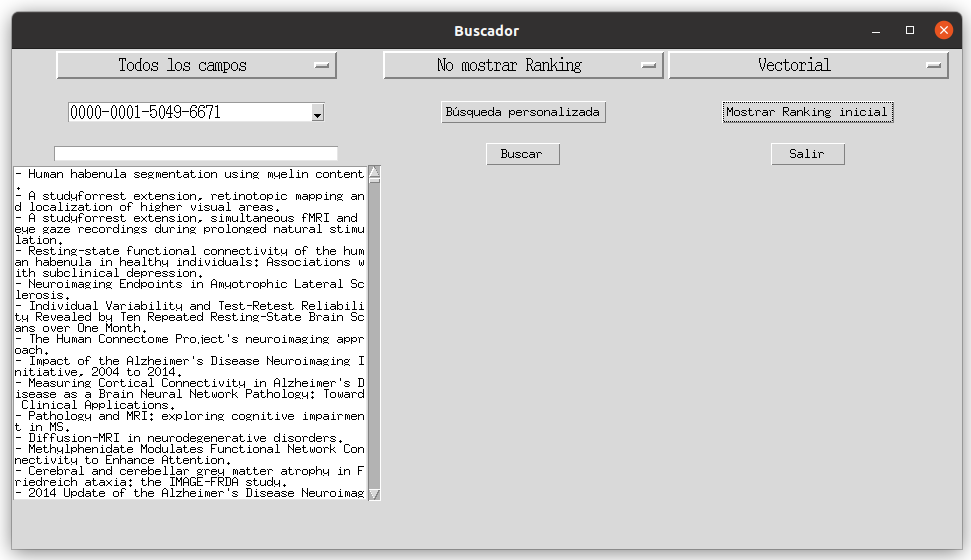
\includegraphics[width=1.0\textwidth]{pg}
\caption{Resultado del algoritmo PageRank.}
\end{figure}

Por último, en cualquier consulta podemos mostrar los pesos de esta, para ello se selecciona en la pestaña ``Mostrar Ranking'' para mostrarlo y ``No mostrar Ranking'' para ocultarlo.
\begin{figure}[H]
\centering
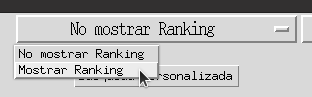
\includegraphics[width=0.8\textwidth]{mostrarranking}
\caption{Desplegable para elegir so mostrar el ranking o no.}
\end{figure}
Los pesos se moestraría de la siguiente forma.
\begin{figure}[H]
\centering
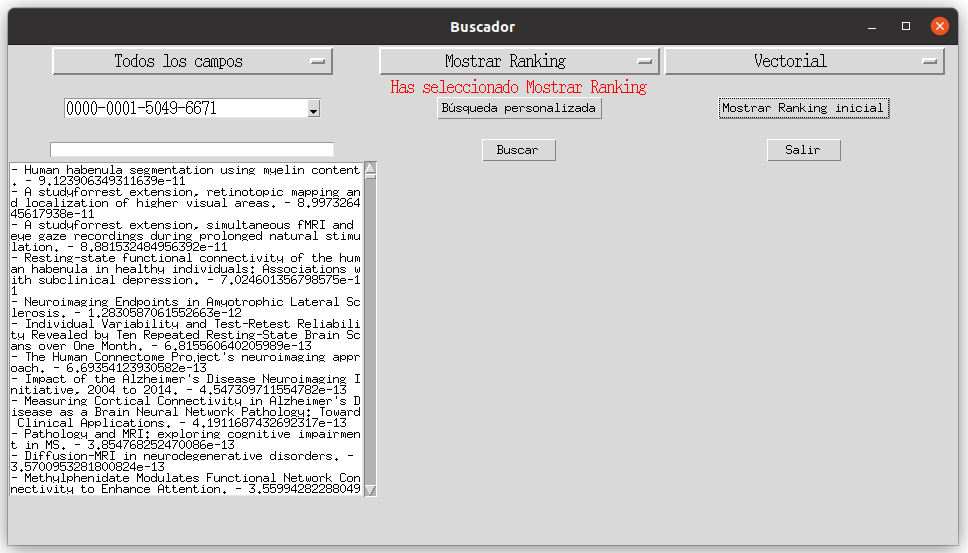
\includegraphics[width=1.0\textwidth]{pgconranking}
\caption{Ranking inicial con los pesos del ranking.}
\end{figure}

\newpage

\section{Esquema de las consultas}
Como se ha comentado anteriormente según el modelo en el se encuentre el sistema la consulta debe introducirse de una forma o de otra.
\begin{itemize}
\item \textbf{\underline{Modelo booleano}}. En este modelo se debe seguir el esquema de la lógica booleana la cual cumple las siguiente reglas:
\begin{itemize}
\item Los operadores binarios (AND y OR) deben aparecer entre dos términos. En caso de que la consulta no lo cumpla se mostrará el siguiente error.
\begin{figure}[H]
\centering
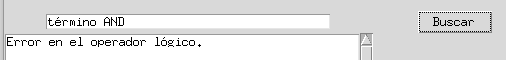
\includegraphics[width=1.0\textwidth]{erroroperador}
\caption{Mensaje de error en el operador lógico.}
\end{figure}
\begin{figure}[H]
\centering
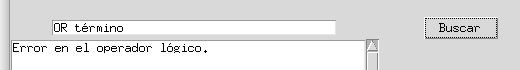
\includegraphics[width=1.0\textwidth]{erroror}
\caption{Mensaje de error en el operador lógico.}
\end{figure}
\item En el caso del operador unario NOT el término a consultar debe ir precedido por el operador. En caso contrario se mostrará el siguiente error.
\begin{figure}[H]
\centering
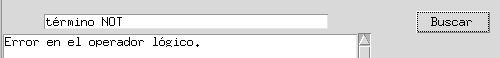
\includegraphics[width=1.0\textwidth]{errornot}
\caption{Mensaje de error en el operador lógico.}
\end{figure}
\item Al combinar los dos operadores, el operador unario debe ir precedido del operador binario, en caso contrario también se mostrará un mensaje de error.
\begin{figure}[H]
\centering
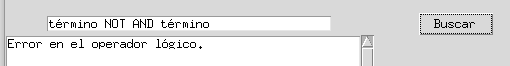
\includegraphics[width=1.0\textwidth]{errororden}
\caption{Mensaje de error en el operador lógico.}
\end{figure}
\item En el caso de anidar esquemas lógicos y de utilizar paréntesis, deberán aparecer el paréntesis de abrir y el de cerrar. En caso contrario, se mostrará un mensaje de error.
\begin{figure}[H]
\centering
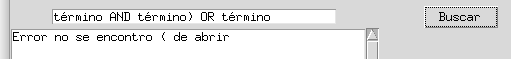
\includegraphics[width=1.0\textwidth]{errorabrir}
\caption{Mensaje de error en los paréntesis.}
\end{figure}
\begin{figure}[H]
\centering
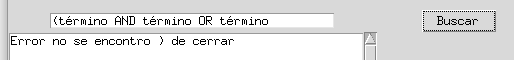
\includegraphics[width=1.0\textwidth]{errorcerrar}
\caption{Mensaje de error en los paréntesis.}
\end{figure}
\item En el caso de querer introducir un término compuesto en la consulta este deberá introducirse entre comillas dobles. En el caso de que no se introduzcan las comillas en alguno de los dos extremos del término se mostrará el error por pantalla.
\begin{figure}[H]
\centering
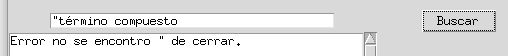
\includegraphics[width=1.0\textwidth]{errorcomillas}
\caption{Mensaje de error en las comillas dobles.}
\label{errorcomillasdobles}
\end{figure}
\end{itemize}
\item \textbf{\underline{Modelo vectorial}}. En este modelo las consultas no tienen ninguna restricción. También se pueden introducir términos compuestos, como en el anterior modelo, introduciendo estos términos entre comillas, en el caso de que el usuario se olvide de cerrar las comillas el sistema mostrará un mensaje de error (Figura \ref{errorcomillasdobles}).

\end{itemize}

\newpage

\section{Resultados}
En esta sección mostraremos los resultados de varias ejecuciones para verificar que estos son lógicos. Realizaremos distintas pruebas dependiendo de las condiciones de cada modelo.

Para ilustrar mejor los ejemplos elegimos dos archivos, por ejemplo el quinto y el décimo clasificados según el PageRank. Estos son:

\underline{Quinto clasificado}
\begin{itemize}
\item Título: Neuroimaging Endpoints in Amyotrophic Lateral Sclerosis.
\item ORCID autor: 0000-0003-0267-3180
\item Abstract: Amyotrophic lateral sclerosis (ALS) is a progressive neurodegenerative, clinically heterogeneous syndrome pathologically overlapping with frontotemporal dementia. To date, therapeutic trials in animal models have not been able to predict treatment response in humans, and the revised ALS Functional Rating Scale, which is based on coarse disability measures, remains the gold-standard measure of disease progression. Advances in neuroimaging have enabled mapping of functional, structural, and molecular aspects of ALS pathology, and these objective measures may be uniquely sensitive to the detection of propagation of pathology in vivo. Abnormalities are detectable before clinical symptoms develop, offering the potential for neuroprotective intervention in familial cases. Although promising neuroimaging biomarker candidates for diagnosis, prognosis, and disease progression have emerged, these have been from the study of necessarily select patient cohorts identified in specialized referral centers. Further multicenter research is now needed to establish their validity as therapeutic outcome measures.
\item Keywords: 'Amyotrophic lateral sclerosis' 'biomarker.'
  'magnetic resonance imaging' 'motor neuron disease' 'trial'
\end{itemize}

\underline{Decimo clasificado}
\begin{itemize}
\item Título: Pathology and MRI: exploring cognitive impairment in MS.
\item ORCIRD autor: 0000-0002-6378-0070
\item Abstract: Cognitive impairment is a frequent symptom in people with multiple sclerosis, affecting up to 70\% of patients. This article reviews the published association of cognitive dysfunction with neuroimaging findings. Cognitive impairment has been related to focal T2 hyperintense lesions, diffuse white matter damage and corical and deep gray matter atrophy. Focal lesions cannot sufficiently explain cognitive dysfunction in MS; microstructural tissue damage detectable by diffusion tensor imaging and gray matter atrophy are probably at least as relevant. Resting state functional magnetic resonance imaging is increasingly used to investigate the contribution of functional connectivity changes to cognitive function in MS. The fact that at least one third of MS patients are not overtly cognitively impaired despite significant radiographic tissue damage argues for protective factors (brain reserve, cognitive reserve) that require further clarification. It is concluded that the reported correlations between imaging findings and cognitive function do not imply causality. Well conceived and sufficiently powered longitudinal studies are lacking. Such studies would help unravel protective mechanisms against cogniitve decline and identify suitable imaging techniques to monitor cognitive function in individual patients with MS.
\item Keywords: 'cognitive impairment' 'functional connectivity' 'gray matter'
  'magnetic resonance imaging' 'multiple scerosis' 'white matter'
\end{itemize}

\begin{itemize}
\item \textbf{\underline{Modelo booleano}}. Elegimos, por ejemplo, una palabra que esté en los dos documentos, por ejemplo, \textit{sclerosis} y otra palabra que solo aparezca en uno de ellos, por ejemplo, \textit{patients} que solo se encuentra en el segundo documento. Realizamos las siguientes búsquedas.

En primer lugar buscamos solo la palabra \textit{sclerosis} y nos aseguramos de que se muestran los dos documentos. Vemos que efectivamente el documento ``Neuroimaging Endpoints in Amyotrophic Lateral Sclerosis'' aparece en primera posición, mientras que el documento ``Pathology and MRI: exploring cognitive impairment in MS'' aparece en tercera posición.

\begin{figure}[H]
\centering
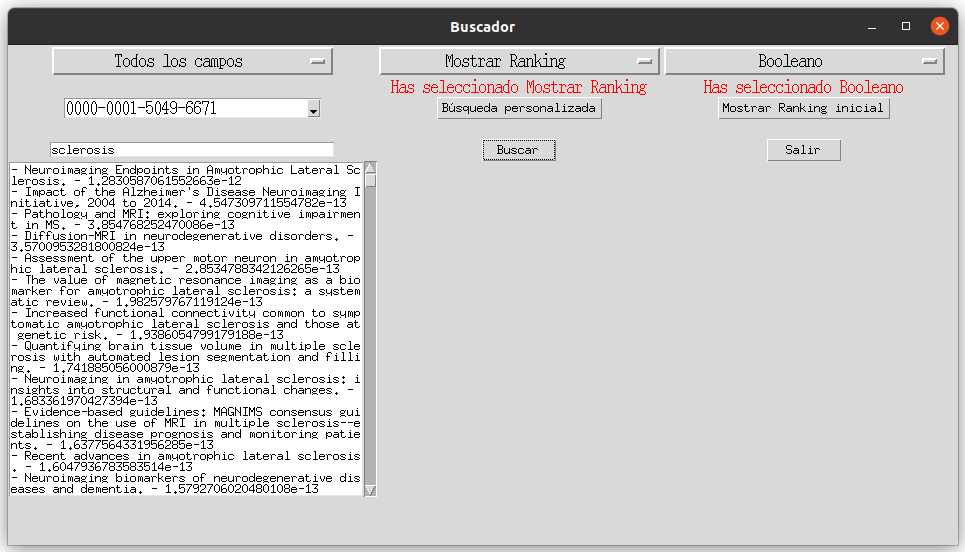
\includegraphics[width=1.0\textwidth]{consulta}
\caption{Resultado de la consulta \textit{sclerosis}.}
\label{errorcomillas}
\end{figure}
A continuación realizamos la consulta \textit{sclerosis AND patients}. Y comprobamos que efectivamente de los dos documentos solo aparece el documento ``Pathology and MRI: exploring cognitive impairment in MS''.
\begin{figure}[H]
\centering
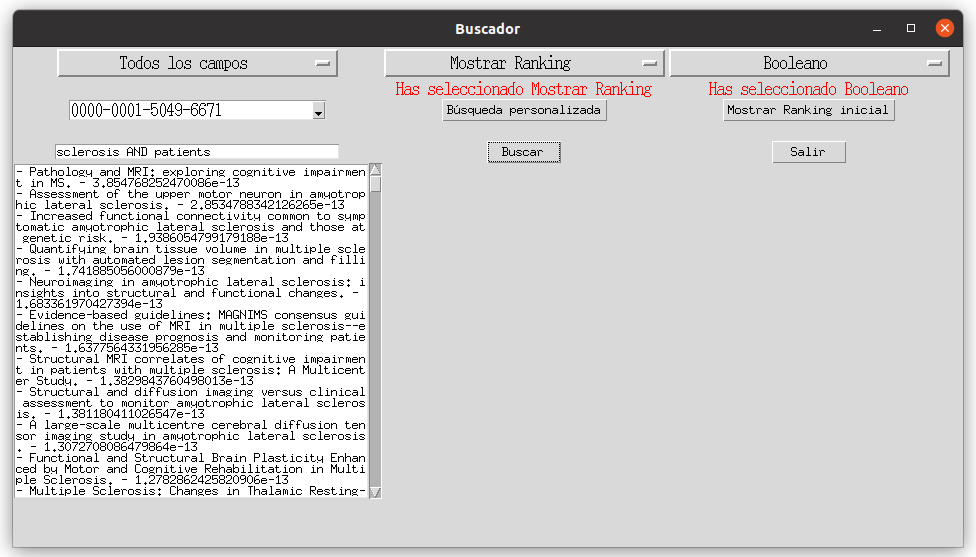
\includegraphics[width=1.0\textwidth]{consultaAND}
\caption{Resultado de la consulta \textit{sclerosis AND patients}.}
\label{errorcomillas}
\end{figure}

Probamos a realizar la consulta \textit{sclerosis AND NOT patients}. Comprobamos ahora que de los dos documentos solamente aparece ``Neuroimaging Endpoints in Amyotrophic Lateral Sclerosis''

\begin{figure}[H]
\centering
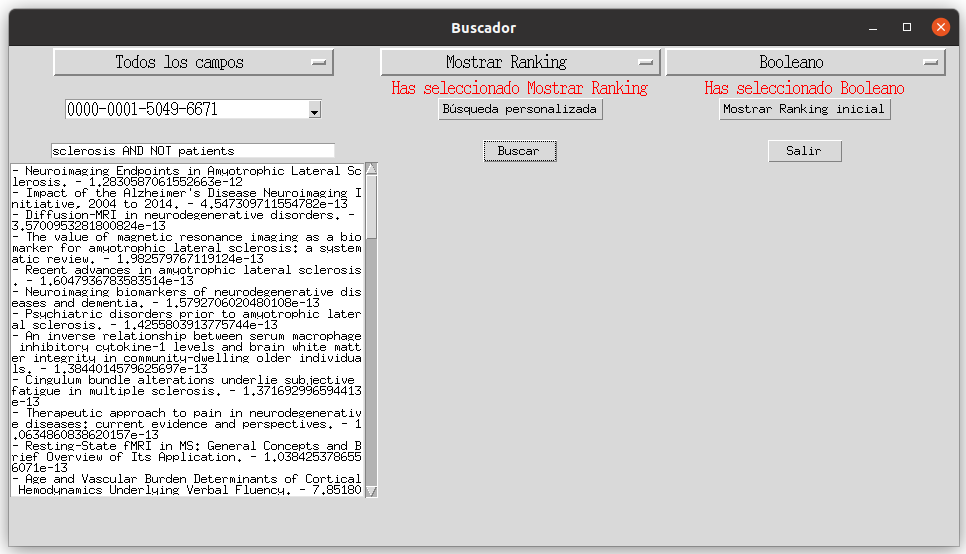
\includegraphics[width=1.0\textwidth]{consultaNOT}
\caption{Resultado de la consulta \textit{sclerosis AND NOT patients}.}
\label{errorcomillas}
\end{figure}

Elegimos ahora una palabra que solo se encuentre en el documento ``Neuroimaging Endpoints in Amyotrophic Lateral Sclerosis'', por ejemplo, \textit{neurodegenerative}, y realizamos la consulta \textit{neurodegenerative OR patients}. Comprobamos que efectivamente aparecen los dos documentos, ``Neuroimaging Endpoints in Amyotrophic Lateral Sclerosis'' situado en la primera posición y ``Pathology and MRI: exploring cognitive impairment in MS'' en la tercera.

\begin{figure}[H]
\centering
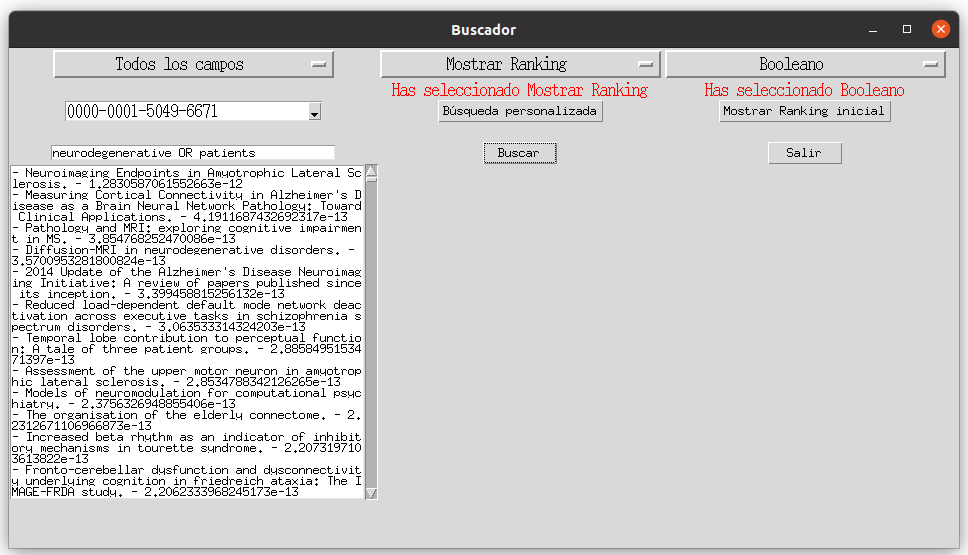
\includegraphics[width=1.0\textwidth]{consultaOR}
\caption{Resultado de la consulta \textit{neurodegenerative OR patients}.}
\label{errorcomillas}
\end{figure}

A continuación seleccionamos que el sistema solo haga la búsqueda en el Título, realizamos la consulta \textit{Sclerosis OR Pathology} y efectivamente aparecen los dos documentos. Uno situado el primero del ranking y el otro situado en tercer lugar.

\begin{figure}[H]
\centering
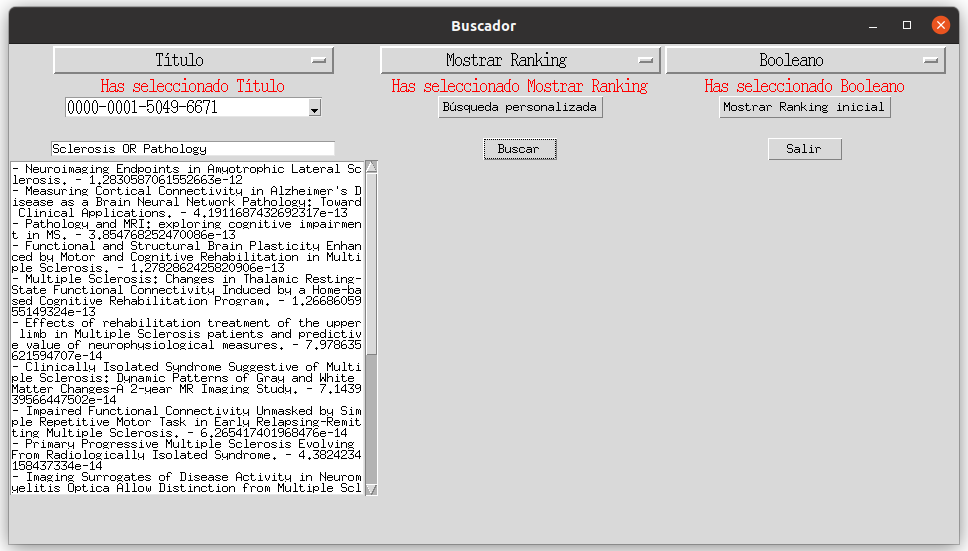
\includegraphics[width=1.0\textwidth]{consultaTitulo}
\caption{Resultado de la consulta \textit{Sclerosis OR Pathology}.}
\label{errorcomillas}
\end{figure}

\item \textbf{\underline{Modelo vectorial}}. Para realizar las pruebas en este modelo utilizaremos los mismos documentos. Realizamos la búsqueda \textit{sclerosis patients} y comprobamos que efectivamente aparecen los dos documentos encabezando el ranking. Vemos que aunque el documento ``Pathology and MRI: exploring cognitive impairment in MS'' contiene las dos palabras, su peso no es suficiente como para superar al otro documento (que solo contiene una palabra), puesto que el peso del orden del PageRank tiene más fuerza (recordemos que es el quinto posicionado según el PageRank mientras que ``Pathology and MRI: exploring cognitive impairment in MS'' es el décimo).

\begin{figure}[H]
\centering
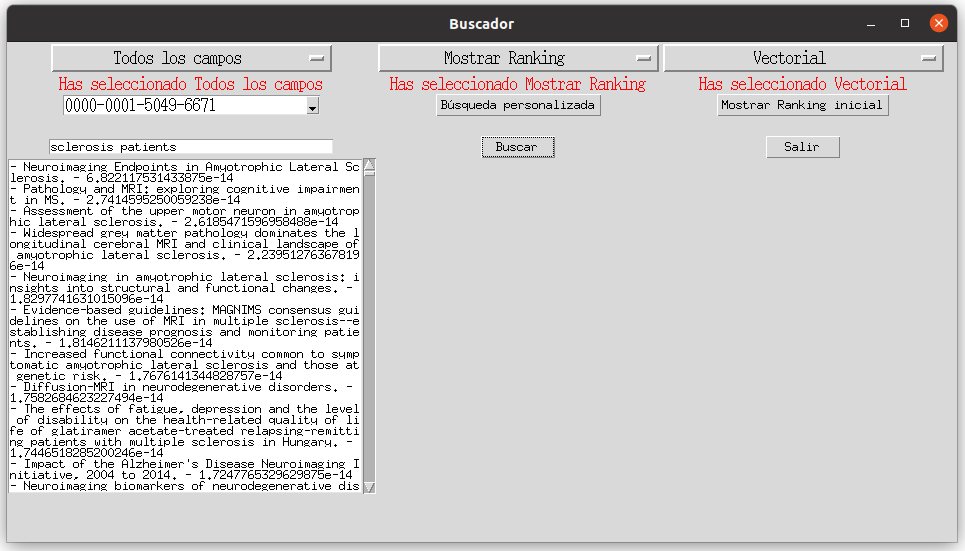
\includegraphics[width=1.0\textwidth]{consultaVEC}
\caption{Resultado de la consulta \textit{sclerosis patients}.}
\label{errorcomillas}
\end{figure}
\end{itemize}

Si a la consulta anterior le añadimos el término \texit{Pathology} conseguimos situar el documento ``Pathology and MRI: exploring cognitive impairment in MS'' por encima de ``Neuroimaging Endpoints in Amyotrophic Lateral Sclerosis'' ya que el primero contiene todas las palabras mientras que el otro solo contiene la palabra \textit{sclerosis}.

\begin{figure}[H]
\centering
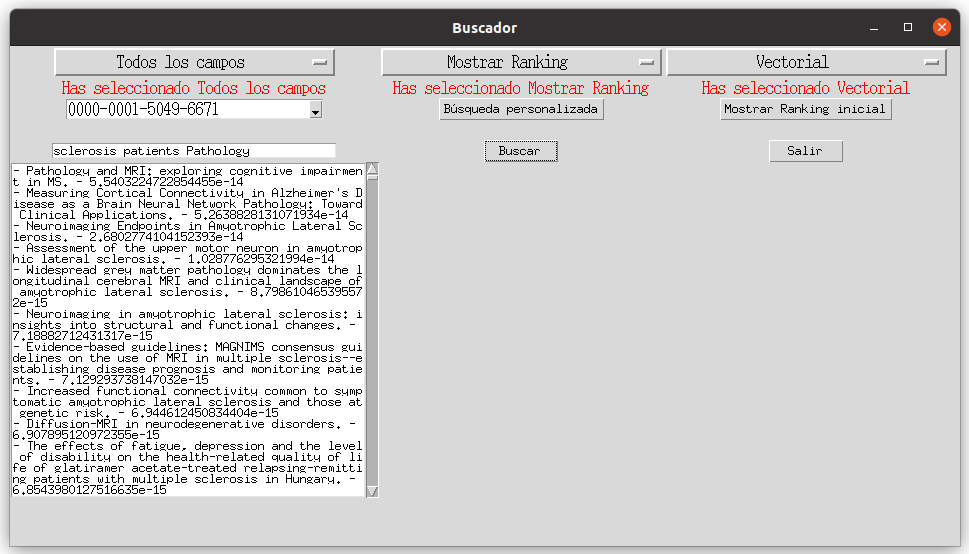
\includegraphics[width=1.0\textwidth]{consultaVEC2}
\caption{Resultado de la consulta \textit{sclerosis patients Pathology}.}
\label{errorcomillas}
\end{figure}
\end{itemize}

Por último, si realizamos la consulta anterior siendo el usuario $0000-0003-0267-3180$, es decir, el autor de ``Neuroimaging Endpoints in Amyotrophic Lateral Sclerosis.'' vemos como este se sitúa por delante del otro documento aún conteniendo menos palabras de la consulta. Habiendo conseguido el propósito de especializar la consulta según el interés del propio usuario.

\begin{figure}[H]
\centering
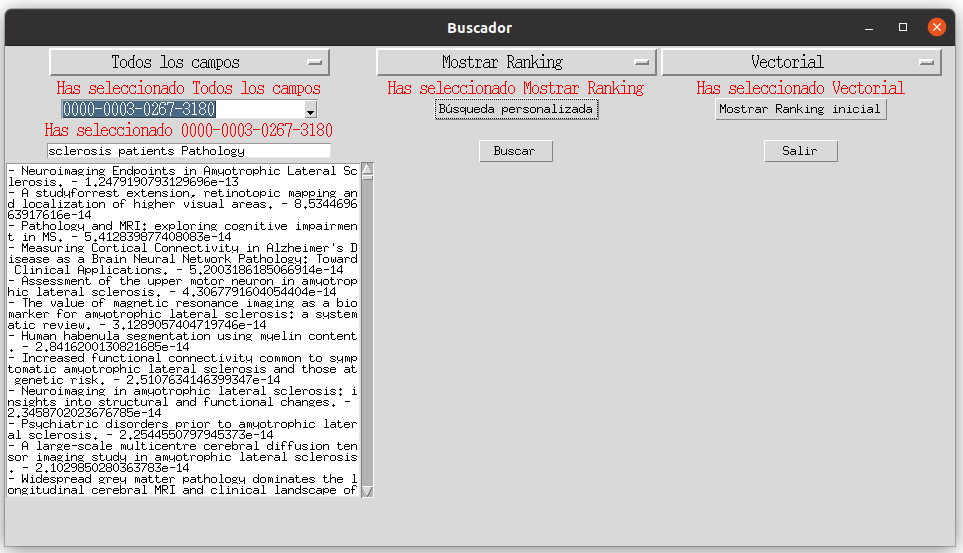
\includegraphics[width=1.0\textwidth]{consultaPER}
\caption{Resultado de la consulta \textit{sclerosis patients Pathology}.}
\label{errorcomillas}
\end{figure}
\end{itemize}

A continuación mostramos los pesos de las distintas consultas del modelo vectorial.

\begin{table}[H]
\centering
\begin{tabular}{|c|c|c|c|c|}
\hline
Consulta                                                                                                      & Título                                                                                               & PageRank  & Similitud & Resultado final \\ \hline
\multirow{2}{*}{"sclerosis patients"}                                                                         & \begin{tabular}[c]{@{}c@{}}Neuroimaging Endpoints in \\ Amyotrophic Lateral Sclerosis\end{tabular} & 1.283e-12 & 0.0532    & 6.822e-14       \\ \cline{2-5}
                                                                                                              & \begin{tabular}[c]{@{}c@{}}Pathology and MRI: exploring \\ cognitive impairment in MS\end{tabular} & 3.855e-13 & 0.0711    & 2.741e-14       \\ \hline
\multirow{2}{*}{\begin{tabular}[c]{@{}c@{}}"sclerosis patients \\ Pathology"\end{tabular}}                    & \begin{tabular}[c]{@{}c@{}}Neuroimaging Endpoints in \\ Amyotrophic Lateral Sclerosis\end{tabular} & 1.283e-12 & 0.021     & 2.680e-14       \\ \cline{2-5}
                                                                                                              & \begin{tabular}[c]{@{}c@{}}Pathology and MRI: exploring \\ cognitive impairment in MS\end{tabular} & 3.855e-13 & 0.144     & 5.540e-14       \\ \hline
\multirow{2}{*}{\begin{tabular}[c]{@{}c@{}}"sclerosis patients \\ Pathology" \\ (personalizada)\end{tabular}} & \begin{tabular}[c]{@{}c@{}}Neuroimaging Endpoints in \\ Amyotrophic Lateral Sclerosis\end{tabular} & 1.283e-12 & 0.973     & 1.248e-13       \\ \cline{2-5}
                                                                                                              & \begin{tabular}[c]{@{}c@{}}Pathology and MRI: exploring \\ cognitive impairment in MS\end{tabular} & 3.855e-13 & 0.14041    & 5.413e-14       \\ \hline
\end{tabular}
\end{table}

\begin{figure}[H]
\centering
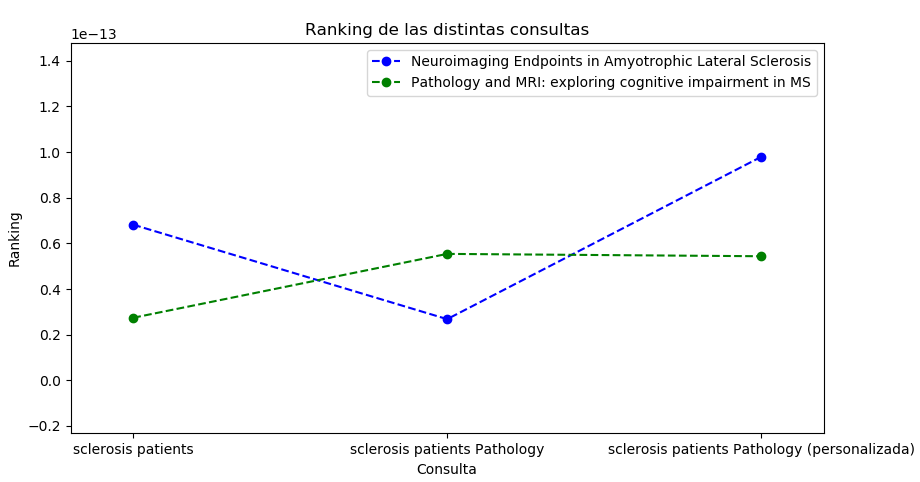
\includegraphics[width=1.0\textwidth]{grafica}
\caption{Ranking de las consultas del modelo vectorial.}
\label{errorcomillas}
\end{figure}

Para analizar la bondad de los resultados utilizaremos dos métricas extraídas de \cite{ri}, entre las cuales existe una relación inversa:
\begin{itemize}
\item Exhaustividad. Se define como la proporción de documentos relevantes que son recuperados en respuesta a una consulta.
$$\textrm{Exhaustividad} = \frac{\textrm{número de docs relevantes recuperados}}{\textrm{número de docs relevantes en la colección}} $$
\item Presición. Se define como la proporción de documentos recuperados que son relevantes en respuesta a una consulta.
$$\textrm{Precisión} = \frac{\textrm{número de docs relevantes recuperados}}{\textrm{número de docs recuperados}} $$
\end{itemize}


Calculamos estos valores para la última consulta donde los documentos relevantes para el usuario que la realiza (el autor $0000-0003-0267-3180$) son los siguientes 25 documentos:
\begin{itemize}
\item Diffusion imaging of whole, post-mortem human brains on a clinical MRI scanner.
\item Multiple kernel learning captures a systems-level functional connectivity biomarker signature in amyotrophic lateral sclerosis.
\item Neuroimaging in amyotrophic lateral sclerosis.
\item Widespread grey matter pathology dominates the longitudinal cerebral MRI and clinical landscape of amyotrophic lateral sclerosis.
\item Magnetoencephalography.
\item Diagnostic accuracy of diffusion tensor imaging in amyotrophic lateral sclerosis: a systematic review and individual patient data meta-analysis.
\item Myelin imaging in amyotrophic and primary lateral sclerosis.
\item Differential corticospinal tract degeneration in homozygous 'D90A' SOD-1 ALS and sporadic ALS.
\item Increased functional connectivity common to symptomatic amyotrophic lateral sclerosis and those at genetic risk.
\item Neuroimaging Endpoints in Amyotrophic Lateral Sclerosis.
\item Voxel-based MRI intensitometry reveals extent of cerebral white matter pathology in amyotrophic lateral sclerosis.
\item Eye-tracking in amyotrophic lateral sclerosis: A longitudinal study of saccadic and cognitive tasks.
\item Corpus callosum involvement is a consistent feature of amyotrophic lateral sclerosis.
\item Does variation in neurodegenerative disease susceptibility and phenotype reflect cerebral differences at the network level?
\item What does imaging reveal about the pathology of amyotrophic lateral sclerosis?
\item Fractional anisotropy in the posterior limb of the internal capsule and prognosis in amyotrophic lateral sclerosis.
\item Quantifying disease progression in amyotrophic lateral sclerosis.
\item A large-scale multicentre cerebral diffusion tensor imaging study in amyotrophic lateral sclerosis.
\item Assessment of the upper motor neuron in amyotrophic lateral sclerosis.
\item Whole-brain magnetic resonance spectroscopic imaging measures are related to disability in ALS.
\item Mind the gap: the mismatch between clinical and imaging metrics in ALS.
\item Psychiatric disorders prior to amyotrophic lateral sclerosis.
\item Mechanisms, models and biomarkers in amyotrophic lateral sclerosis.
\item Controversies and priorities in amyotrophic lateral sclerosis.
\item EFNS guidelines on the use of neuroimaging in the management of motor neuron diseases.
\end{itemize}

De los cuales en la consulta \textit{sclerosis patients Pathology} aparecen 24, por lo tanto:
$$\textrm{Exhaustividad} = \frac{\textrm{número de docs relevantes recuperados}}{\textrm{número de docs relevantes en la colección}} = \frac{24}{25} = 0.96 $$
Por otro lado en la consulta \textit{sclerosis patients Pathology} se recuperan 2141 documentos, por lo tanto la \textit{Presición} será la siguiente:
$$\textrm{Precisión} = \frac{\textrm{número de docs relevantes recuperados}}{\textrm{número de docs recuperados}} = \frac{24}{2141} = 0.0112$$

Viendo los datos anteriores podemos concluir que nuestro sistema es bastante exhaustivo, pero poco preciso, resultado lógico ya que entre las dos métricas existe una relación inversa. Es decir, nuestro buscador consigue recuperar la mayoría de los archivos relevantes, aunque en el proceso aparecen también muchos documentos no relevantes. Sería interesante, para trabajos futuros, lograr mejorar la precisión del buscador modificando los pesos del algoritmo.

\newpage
\section{Conclusiones y trabajos futuros}
Se han alcanzado los objetivos propuestos ya que se resuelve el problema inicial de ordenar información según el interés del usuario. El método de las potencias proporciona una buena aproximación de la solución buscada.
Por otro lado, el algoritmo PageRank obtiene resultados bastante buenos a la hora de ordenar los archivos por relevancia. Además los modelos implementados también obtienen buenos resultados, consiguiendo además personalizar las búsquedas.

El algoritmo PageRank, como es bien conocido, es un algoritmo de gran interés y de aplicación en multitud de campos como hemos podido observar con su utilización en áreas para el que inicialmente no había sido pensado como se ha visto en la búsqueda de referencias bibliográficas. Por otro lado, la implementación de este en el contexto de documentos y términos, me ha iniciado en el área de la Recuperación de Información de la que no tenía ningún conocimiento previo.

Problemas de índole organizativo me han impedido la utilización de un servidor del departamento de CCIA de mayor capacidad para la explotación del sistema con la colección completa como se había previsto, por lo que me he visto condicionada a reducir considerablemente el conjunto de datos inicial.

Sería interesante, como futuros proyectos, crear perfiles de usuario con distintos intereses para poder personalizar mejor la búsqueda, consiguiendo mostrar en los primeros resultados los archivos más importantes para el usuario dependiendo de su perfil. Además, también se podría modificar el software para que se amoldarse a otra colección de datos, buscando que la interfaz sea capaz de adaptarse automáticamente a la estructura de estos. Otra posible ampliación, sería la paralelización del algoritmo buscando como objetivo adaptar el software a conjuntos de datos más grandes. Por último también sería interesante conseguir mejorar la precisión de nuestro actual sistema ajustando los pesos del modelo.




\newpage

\begin{thebibliography}{9}
\bibitem{algebralineal}
Carl D. Meyer.
\textit{Matrix Analysis and Applied Linear Algebra}. Siam. 2000.

\bibitem{jordan}
Luis Merino y Evangelina Santos.
\textit{Álgebra lineal con métodos elementales}. Paraninfo. 1999.

\bibitem{modelos}
Rafael Ortega Rios.
\textit{Modelos matemáticos}. Editorial Universidad de Granada. 2013.

\bibitem{ri}
Fidel Cacheda Seijo, Juan Manuel Fernández Luna y Juan Francisco Huete Guadix.
\textit{Recuperación de Información. Un enfoque práctica y multidisciplinar}. RA-MA Editorial y Publicaciones. 2011.

\end{thebibliography}
%printbibliography

\newpage

\appendix
\section{Guía de uso del código}
La implementación del sistema se ha llevado a cabo en dos archivos \verb|pagerank.py| y \verb|interfazgrafica.py|. El primer fichero contiene el código de todos los algoritmos y modelos implementados, así como la lectura del conjunto de datos PMSC-UGR, mientras que el segundo contiene el código utilizado para la interfaz gráfica en la cual se comunica el usuario con el sistema.

El sistema mostrado en el trabajo se ha ejecutado sobre un subconjunto del conjunto de datos PMSC-UGR. Este subconjunto ha sido previamente procesado originando tres archivos: \verb|vectorPG.csv|, \verb|matrizt.csv| y \verb|matrizw.csv|. En el caso de contar con los archivos y con el subconjunto de la colección de documentos, solo es necesario introducir la ruta de de la carpeta de la carpeta contenedora de los archivos al principio del fichero \verb|pagerank.py|:
\begin{itemize}
\item Para el conjunto de datos, introduciremos la ruta al principio del archivo \verb|pagerank.py| en la variable \verb|BBDPATH| de la siguiente forma:
\begin{verbatim}
BBDPATH = "/home/johanna/Documentos/TFG/base-de-datos/base"
\end{verbatim}
Donde \verb|base| es la carpeta contenedora.
\item Para los archivos ya procesados, introduciremos la ruta de la capeta contenedora de los tres archivos comentados al principio (\verb|vectorPG.csv|, \verb|matrizt.csv| y \verb|matrizw.csv|) al principio del archivo \verb|pagerank.py| en la variable \verb|PATH|:
\begin{verbatim}
PATH = "/home/johanna/Documentos/TFG/implementacion/matrices/"
\end{verbatim}
\end{itemize}
Una vez seleccionado las rutas solo es necesario ejecutar el archivo \verb|interfazgrafica.py| con Python.
\begin{verbatim}
python interfazgrafica.py
\end{verbatim}

En el caso de no tener alguno de los archivos de los datos procesados (\verb|vectorPG.csv|, \verb|matrizt.csv| y \verb|matrizw.csv|) se introducirá en la ruta \verb|PATH| la carpeta donde se desea almacenar la información y se ejecutará el programa con normalidad (\texttt{python interfazgrafica.py}). Esta ejecución puede tardar unas 20 horas, puesto que no están los datos procesados previamente. Tras esta ejecución se almacenarán en la carpeta introducida los datos procesados y comenzará el sistema automáticamente.


\end{document}
